%\documentclass[natbib]{svjour3}
%\documentclass[manuscript]{acmart}
\documentclass[10pt,journal,compsoc]{IEEEtran}
%\documentclass{sig-alternate}
%\documentclass{llncs}

\usepackage{booktabs} % For formal tables
\usepackage[T1]{fontenc}
\usepackage[]{hyperref} %sections as bookmarks in adobe pdf
%\hypersetup{pdfpagelabels=false}
\hypersetup{
	colorlinks = true, %Colours links instead of ugly boxes
	urlcolor   = blue, %Colour for external hyperlinks
	linkcolor  = blue, %Colour of internal links
	citecolor  = blue   %Colour of citations
}

\usepackage{times}
\usepackage{multirow}
\usepackage{wrapfig}
%\usepackage[usenames, dvipsnames]{color}
\usepackage{booktabs}

% Macros for proof-reading & corrections
\usepackage[normalem]{ulem} % for \sout
\usepackage{xcolor,xspace}
% Put edit comments in a really ugly standout display
\usepackage{ifthen}

% Advanced Math
\usepackage{amsmath}
%\usepackage{amssymb}	% double line font letters (for number sets N,Z,D,Q,R)

% Images and Floats
\usepackage{epsfig}
%\usepackage{epstopdf}

\usepackage{caption}
\usepackage{subcaption}
%\usepackage{lscape}			% landscape
%\usepackage{array}			% align vertically in tables
%\usepackage{rotating}


% Theorems, Definitions, ... (always after 'amsmath')
%\let\proof\relax  \let\endproof\relax %amsthm redefined \proof, genereting conflicts.
%\usepackage{amsthm}
%\theoremstyle{definition}
%\newtheorem{prop}{Property}%[section]
%\newtheorem{defn}{Definition}%[section]

% Commutative diagrams
%\usepackage{diagrams}

%\usepackage{enumitem}
\usepackage{graphicx,wrapfig,lipsum}
\usepackage{flushend}



%For code listings:
\usepackage{listings}
% \lstset{language=[OMG]OCL,
\lstset{language=[decorative]OCL,
	basicstyle=\ttfamily,
	keywordstyle=\color{black}\bfseries,
	commentstyle=\textit,
	escapeinside={(*@}{@*)},
	morekeywords={Context, self, closure},
	morecomment=[l]{!\ }% Comment only with space after !
}

%\usepackage[sectionbib,square]{natbib}
\usepackage[square,numbers]{natbib}

%\setlength{\paperheight}{11in}
%%%%%%%%%%%%%%%%%%%%%%%%%%%%%%%%%%%%%%%%%%%%%




% Standard shortcuts
\newcommand{\eg}{\emph{e.g.,~}}							% exempli gratia (for the sake of example)
\newcommand{\ie}{\emph{i.e.,~}}							% id est (that is)
\newcommand{\Fig}[1]{Fig.~\ref{#1}}  			% choose Fig. or Figure, depending on the style
\newcommand{\Table}[1]{Table~\ref{#1}}	    % Table reference
\newcommand{\Sect}[1]{Section~\ref{#1}}	  % section name always with a capital S
\newcommand{\Model}[1]{\textsf{\small{#1}}} % name of any modeling artifact (e.g., formalism, model element, rule, ...)
\newcommand{\Code}[1]{\texttt{\small{#1}}}	% inline code
\providecommand{\e}[1]{\ensuremath{\times 10^{#1}}}	% scientific notation: x.10^y

%%%%%%%%%%%%%%%%%%%%%%%%%%%%%%%%%%%%%%%%%%%%%

% Shortcuts
\newcommand{\MOF}{\textsc{MOF}\xspace}
\newcommand{\ocl}{\textsc{OCL}\xspace}
\newcommand{\OCL}{\textsc{OCL}\xspace}
\newcommand{\nsga}{\textsc{NSGA-II}\xspace}
\newcommand{\MDE}{\textsc{MDE}\xspace}
\newcommand{\MT}{\textsc{MT}\xspace}
\newcommand{\WFR}{\textsc{WFR}\xspace}
\newcommand{\Ecore}{\textsc{Ecore}\xspace}
\newcommand{\OURNAME}{{our approach}\xspace}



\newcommand{\ra}{$\rightarrow$}
\newcommand{\la}{$\leftarrow$}
\newcommand{\ugh}[1]{\textcolor{red}{\uwave{#1}}} % please rephrase
\newcommand{\ins}[1]{\textcolor{blue}{\uline{#1}}} % please insert
\newcommand{\del}[1]{\textcolor{red}{\sout{#1}}} % please delete
\newcommand{\chg}[2]{\textcolor{red}{\sout{#1}}{\ra}\textcolor{blue}{\uline{#2}}} % please change
\newcommand{\move}[2]{\textcolor{blue}{\uwave{#1} (Move to #2)}} % please move


\newboolean{showcomments}
\setboolean{showcomments}{true} % toggle to show or hide comments
\ifthenelse{\boolean{showcomments}}
{\newcommand{\nb}[2]{
		\fcolorbox{gray}{yellow}{\bfseries\sffamily\scriptsize#1}
		{$\blacktriangleright$#2$\blacktriangleleft$}
	}
	\newcommand{\version}{\emph{\scriptsize$-$working$-$}}
}
{\newcommand{\nb}[2]{}
	\newcommand{\version}{}
}



\newcommand\eb[1]{\nb{EB}{\textcolor{red}{\textsl{#1}}}}
\newcommand\jc[1]{\nb{JC}{\textcolor{red}{\textsl{#1}}}}
\newcommand{\todo}[1]{\textbf{\textcolor{red}{TODO: #1}}}
\newcommand\syn[0]{\fcolorbox{gray}{green}{\bfseries\sffamily\scriptsize{SYN.}}}

\newcommand\bluefat[1]{$\blacktriangleright$\textcolor{blue}{\textit{#1}}$\blacktriangleleft$}
\newcommand\blue[1]{\textcolor{blue}{#1}}
\newcommand\red[1]{\textcolor{red}{#1}}

\makeatletter
\def\ughu{\bgroup \markoverwith{\lower3.5\p@\hbox{\sixly \textcolor{red}{\char58}}}\ULon}
\font\sixly=lasy6 % does not re-load if already loaded, so no memory problem.
\makeatother


\newcommand\missref[1]{\ughu{#1}~\ugh{[?]}}
% Copyright
%\setcopyright{none}
%\setcopyright{acmcopyright}
%\setcopyright{acmlicensed}
%\setcopyright{rightsretained}
%\setcopyright{usgov}
%\setcopyright{usgovmixed}
%\setcopyright{cagov}
%\setcopyright{cagovmixed}


% DOI
%\acmDOI{10.1145/nnnnnnn.nnnnnnn}

% ISBN
%\acmISBN{978-x-xxxx-xxxx-x/YY/MM}



\begin{document}


\title{A Survey-driven Feature Model for Software Traceability Approaches} 
%\title[]{Explainable AI with traceability for the Model-Driven perspective} 
%\titlerunning{Explainable AI with traceability for MDE}        % if too long for running head
%\title[]{The quest for omniscience leads to ubiquitous traceability.} 


%Authors IEEE tran
\author{\IEEEauthorblockN{Edouard Batot}
	\IEEEauthorblockA{SOM-UOC
		ebatot@uoc.edu\\}
	\and
	\IEEEauthorblockN{Sebastien Gerard}
	\IEEEauthorblockA{CEA~LIST
	sebastien.gerard@cea.fr\\}
\and
	\IEEEauthorblockN{Jordi Cabot}
	\IEEEauthorblockA{ICREA \& UOC
	jordi.cabot@icrea.cat\\}
}
%FIN Authors IEEE tran


%\author{Edouard Batot}
%\affiliation{%
%	\institution{UOC}
%%	\streetaddress{P.O. Box 1212}
%%	\city{Dublin} 
%%	\state{Ohio} 
%%	\postcode{43017-6221}
%}
%\email{ebatot@uoc.edu}
%
%%\author{Matteo Morelli}
%%\authornote{Dr.~Trovato insisted his name be first.}
%%\orcid{1234-5678-9012}
%%\affiliation{%
%%	\institution{CEA List}
%	%	\streetaddress{P.O. Box 1212}
%	%	\city{Dublin} 
%	%	\state{Ohio} 
%	%	\postcode{43017-6221}
%%}
%%\email{matteo.morelli@cea.fr}
%\author{Sebastien Gerard}
%%\authornote{Dr.~Trovato insisted his name be first.}
%%\orcid{1234-5678-9012}
%\affiliation{%
%	\institution{CEA List}
%	%	\streetaddress{P.O. Box 1212}
%	%	\city{Dublin} 
%	%	\state{Ohio} 
%	%	\postcode{43017-6221}
%}
%\email{sebastien.gerard@cea.fr}
%\author{Jordi Cabot}
%%\authornote{Dr.~Trovato insisted his name be first.}
%%\orcid{1234-5678-9012}
%\affiliation{%
%	\institution{ICREA-UOC}
%%	\streetaddress{P.O. Box 1212}
%%	\city{Dublin} 
%%	\state{Ohio} 
%%	\postcode{43017-6221}
%}
%\email{jcabot@uoc.edu}

\IEEEtitleabstractindextext{%
	\begin{abstract}
Traceability is the capability to represent, understand and analyze the relationships between software artefacts. Traceability is at the core of many software engineering activities. This is a blessing in disguise as traceability research is scattered among various research subfields which impairs a global view and integration of the different innovations around the recording, identification and management of traces. This also limits the adoption of traceability solutions in industry.

In this sense, the goal of this paper is to present a characterization of the traceability mechanism as a feature model depicting the shared and variable elements in any traceability proposal. The features in the  model are derived from a survey of papers related to traceability published in the literature. We believe this feature model is useful to assess and compare different proposals and provide a common terminology and background that could speed up the creation of new ones on top of them. Beyond the feature model, the survey we conducted also help us to identify a number of challenges to be solved in order to move traceability forward, especially in a context where, due to the increasing importance of AI techniques in Software Engineering, traces are more important than ever in order to be able to reproduce and explain AI decisions.


%Developing techniques to facilitate the representation and analysis of software and system artefacts has always been under the scrutiny of researchers. More particularly, tracing links between related artefacts has shown significant value. Traceability helps explaining the execution and evolution of software systems and assists the progress of primary software engineering disciplines such as program understanding, maintenance, and debugging.
%Yet, the results of traceability investigations are scattered among various research fields and a common ground for theorizing and conceptualizing traceability remains slow to emerge. This is, at least in part, due to a lack of interest from stakeholders as well as remaining of the idea that traceability is of no use to software development efficiency and quality.
%In this paper, we argue that the many purposes traces enable to software engineers share a strong common base. We gather them in a feature model that aims to help readers understand all the dimensions they should keep in mind when evaluating traceability approaches. We ground our approach on a methodological selection of publications referring to the modeling of tracing abilities as well as to tracing itself.% to derive commonalities among features and dimensions.

\end{abstract}

% Note that keywords are not normally used for peerreview papers.
%\begin{IEEEkeywords}
%Computer Society, IEEEtran, journal, \LaTeX, paper, template.
%\end{IEEEkeywords}}


	
	% Note that keywords are not normally used for peerreview papers.
	\begin{IEEEkeywords}
		Software Engineering, Model-Driven Development, Traceability, Feature Model, Explainability
	\end{IEEEkeywords}
}
 


\maketitle

%\hrulefill
\section{Introduction} \label{sec:intro}

The need for traceability has always been salient in software and systems development. Across the years, there has been a continuous interest in developing techniques to facilitate the representation and analysis of traces and links between related artefacts. It helps explaining their execution and evolution as required  in many software engineering activities and disciplines such as code-generation, program understanding, software maintenance, and debugging. 

The importance of traceability was first recognized in system engineering especially related to the development and certification of critical systems where it is a primary concern. As an example, traceability is part of any certification mechanism in all commercial software-based aerospace systems as stated in documents like the RTCA DO-178C (2012)~\cite{paz2019-Modelling-Avionics-Certification,moy2013-DO-178C-testing}. The consideration of various levels of abstraction in software development and the meaning of verification in model-based development paradigm - which figures abstract representations (models) as the core artefact for conceptualization -  was latter introduced with companion documents (specifically, DO-331). The automotive industry has followed the same path with the construction of an international standard for functional safety~\cite{iso26262}. %At code, requirement, model, human and organisational level, a cross-sectorial view provided through traces of processes' executions and artefacts' dependencies figures an ideal tool support for software development and maintenance.

Despite these important evidences on the need for explicit (and automated) tracing abilities in software development, traceability is not widely adopted, even less automated, and there is little feedback from its concrete use in industry~\cite{panis2010-req-traceability-deployment-in-commercial-engineering-organisation} beyond the critical domains above. 

There is a lack of global techniques to ease the manipulation of traces and automate tracing processes. Thereby, traceability in the industry, when required, ends up being mostly a manual process~\cite{mader2009-motivation-matters-in-traceability-practitioner-survey}.
%Winkler \textit{et al.} show all the disregard such "mandatory" characteristic implies - expressly to safety critical software demanding a legal assessment or certification to run~\cite{winkler2010-survey-traceability-and-MDE}. Mader \textit{et al.} show that the benefits of automated traceability is still to be justified to stakeholders who still prefer the burden of \textit{ad hoc} and manual trace elicitation~\cite{mader2009-motivation-matters-in-traceability-practitioner-survey}. 
Moreover, with no standard definition or representation of traces, it is difficult to bridge the gaps between the different partial traceability solutions existing in research subfields\cite{antoniol2017-traceability-grand-challenges,wohlrab2020-traceability-organization-process-culture,winkler2010-survey-traceability-and-MDE}.   %a gap remains between broader fields of investigation beneficial from automated tracing ability (\textit{e.g.,} requirement engineering, program understanding, testing). As a matter of fact, 
Even the software engineering body of knowledge do not seem to properly consider the key relevance of traceability in software engineering as it only mentions traceability once~\cite{swebok2014}.
%Many studies suggest that there is a lack of synthetic and systematic investigations on traceability and research is scattered among many sub-fields. This lack of a common tool for communication hampers sharing between research teams~

All this in a context where artificial intelligence techniques are being integrated in development processes, raising the need for more powerful reproducibility and explainability concerns, both requiring the assistance of traceability mechanisms. %and therefore explainability needs are increasing. Yet, there exists no silver bullet to solve the different expectations brought by tracing ability. Approaches vary greatly in their means and goals. The foundation for an effective modelling of traceability is disseminated among a profuse literature. Moreover, most approaches focus on specific pairs of artefacts and therefore remain difficult to integrate in industrial scenarios.

%the paper aims to help readers understand all the dimensions they should keep in mind when evaluating traceability approaches.
This paper aims to provide a comprehensive perspective on the state of the art of traceability techniques in software development and their limitations with the short-term goal of facilitating the evaluation and comparison of current solutions. And with the mid-term goal of accelerating the development of new traceability solutions that could benefit from the existing ones thanks to our new conceptualization in the form of a feature model describing the potential dimensions and concerns a traceability solution may wish to consider.   %We ground our work with a survey that target publications involved in the modelling of traceability to reflect on the emergence of the field.
%This is the motivation to classify papers according to a series of dimensions that should facilitate the creation (or combination) of more powerful traceability solutions in the future. To help compare current and future traceability proposals we provide a feature model that aims to organize and structure the main traceability concepts. 
We do not create the feature model or just based on our (partial) knowledge and expertise in the domain. Instead, we ground our classification with a survey of the published literature in this field. According to this survey, we group the traceability features in three main dimensions: trace definition, trace identification and trace management, with the corresponding feature hierarchies for each of them. 

%[Metamodeling needed for communication~\cite{winkler2010-survey-traceability-and-MDE}]
%[Metmodeling ISO/IEC 24744:2007 does not mention traceability.\ugh{Check 24744:2014}]

The paper is organized as follows. After a brief introduction, we discuss in \Sect{sec:soa} how our work compares to other meta studies and characterizations of traceability research. We then introduce some basic traceability terminology in \Sect{sec:terminology}. Section~\ref{sec:survey} describes how we conducted our literature review and \Sect{sec:fm} presents a detailed feature model derived from the survey of the retrieved works. This analysis also helps us to propose a number of discussion points and open challenges in \Sect{sec:discussion} before concluding this work. 


\subsection{State of the art} \label{sec:rw}
We present and discuss in this section works related to ours to motivate and justify the need of a new survey in this field. %We will start by exposing the meta-studies dealing with the literature relating to traceability approaches in general. Then, we will present the meta-studies whose purpose is to make the state of the art of approaches using artificial intelligence to assist in the identification of trace links. 

An initial survey of the work done to increase the automation of traceability in software systems was published in 2007 with a great impact~\cite{clelandhuang2007bestPracticeForAutomatedTraceability}. Authors describe nine best practices to augment the potential of traceability that will remain until today the long reach goal to achieve in the emerging research community. They call for a clear establishment of traceability purposes. They also call for an effort from researchers to define the granularity they need to achieve their goals. Researchers must as well keep in mind what will require the integration of this ideal tooling into native software environments. 
On a concrete level, requirement traceability needs quality specifications and exact term definitions to express clearly the conceptualization occurring among them. This requires rich content. Rich enough to bridge the cognitive gaps that plague transitions from one lifecycle phase to the next. Rich enough as well to connect intra-domain semantic synonyms and keep a coherent hierarchy between traced concepts. 
The same year, Galvao \textit{et al.} surveys approaches addressing MDE limitations regarding traceability~\cite{galvao2007-survey-traceability-in-MDE}. In this work, authors show the enormous potential of MDE to represent traces, to generate them automatically, and to assist their management and maintenance. MDE is a suitable paradigm to reach for the end-to-end traceability ideal. Authors describe in great details on the usages of traceability in MDE in a distinctive comparison of the different existing approaches. They conclude that a lack in design and specification modeling, as well as a lack in traceability metamodeling, hampers the automation of traceability techniques through the software life cycle in the MDE paradigm. 

These synthetic works preceded a peak in the number of investigations mentioning explicitly traceability. (In \Fig{fig:publicationyears-tm}, we see that in 2010 22 studies mentioned traceability and modeling.) 
Among them, Winkler \textit{et al.} published an in-depth exploration of both traceability in requirement engineering and model-based development~\cite{winkler2010-survey-traceability-and-MDE}. 
Authors point out that researchers in the two research fields do not communicate enough between each others. This hampers the establishment of common rich and ubiquitous traceability techniques. The authors points out at a lack of tooling in a field where everything is set to support automated traceability. Automated transformations are the very best soil to grow end-to-end traceability at a core level. Yet, even in the modeling community, traceability practices are consider far from mature. There is ongoing research to model the traceability process, but there lacks a pro-active sharing between the larger communities researchers belong to (such as requirement engineering, program understanding, and so on). This piece of work is the closest to ours and we aim at continuing this work with taking account of new trends and describing a more functional approach.

Since studies dedicated to traceability come from specific areas, the general understanding is long to converge. All and every literature synthesis call for more common terminology to allow the sharing of scientific results and help augment the maturity of the emerging research field~\cite{winkler2010-survey-traceability-and-MDE}. On an industrial perspective, some industrial interviewees did not even know what traceability actually is about and rose concerns about its salience during the development process~\cite{vale2017-SPL-traceability-a-SMS,clelandhuang2014-traceability-trends-and-futurte-direction}. Traceability is a major concern in the development of safety critical system, but since it is mandatory it does not gain much enthusiasm. As Mader \textit{et. al.} show in their work, traceability has been considered poorly (by non-traceability stakeholders and researchers) and would benefit a better understanding of its purposes. This would help gather evidences (if they still lack) of the importance of tracing abilities during software development and maintenance~\cite{mader2009-motivation-matters-in-traceability-practitioner-survey}. 

Based on these previous works and the disruptive popularity of AI in software engineering, we believe there is a need for a survey that: 1- summarizes and reflects on the changes and new proposals in the last decade and 2 - goes beyond describing the proposals and makes an effort to synthesize their information in a common traceability glossary, metamodel and feature model to help better characterize the area, application scenarios and potential impact on the growing field of AI-enabled software engineering.

%We try to overcome the aforementioned limitations by proposing a complete study comprising a description of the hierarchy of concepts related to traceability, an articulation of the existing configurations coming from the various engineering domains in which traceability participates, and a holistic characterization of traceability application domains. In this sense, our paper differs from previous research as it offers an actionable view of traceability features and purposes. 





%\section{Motivation}\label{sec:motivation}

To illustrate better the relevance and challenges of implementing traceability appraoches in practice, \ugh{especially in complex CPS environments}, we motivate our words with concrete industrial examples in safety critical software development. We introduce three experiences from our \nb{First mention}{industrial partner} as concrete examples of limitations of current traceability practice.  


\subsection{Manual preference}
Stakeholders and lead architects are unanimous about the need for a robust, accurate, and agile tracing potential through software life cycle. As a matter of fact, it is obvious to any interlocutor that a tool able to elicit any link between two or more artefact from a software system (documentation, certification, code, configuration, design, test, and so on.) is a must for prevention and maintenance. Yet, this tool has not emerged and tracing activities are performed in an \textit{ad hoc} manner. 
As an example, a quality audit at a supplier of our industrial partner resulted in the manual inspection of a huge amount of artefacts in a system. The massive human workload to extract relevant traces and update loads of spreadsheets to commit to SPICE certification~\cite{SPICE-ISO15504} was preferred to automated approaches available. 


\subsection{Product lifecycle management first}
In sequential development, tracing phases and tasks is explicit. Between each phase, when products are passed from one task to the next figures a check point where constraints can be set to maintain the overall legibility of product, information, and management flows. 
When development becomes collaborative, with concurrent tasks performed in parallel, these check points can no longer survive. Phases and tasks overlap and concurrent versions emerge.
To ensure the quality of the development through the whole life cycle, concurrent collaboration requires tracing abilities between phases and tasks, people, processes, and products~\cite{ghaisas2019-traceability-for-a-knowledge-driven-SW}. 
Yet, when time comes to take a decision on which software is best fit to manage a nuclear plan project, it is clear that a mature tooling with traceability as a core concern is not available. This is unfortunate because it would figure a consequent plus value in this kind of project where safety and security are the most prominent concern. 
To develop internally such a software is not possible either - our partner is not an information technology company, and cannot bare such heavy and complex development. This case involves hundreds actors, dozens industrial partners, and produces hundreds requirements, hundreds software products, and thousands relationship between them.
Alternatively, using a certified software from a trusted vendor makes better return on investment (ROI), requires much less burden, and responsibilities.
Our industrial partner was thus rather inclined to invest in a product lifecycle management (PLM) software, serviced by a leader in software development instead of creating its own traceability-first software product. 

Product lifecycle management tools (PLMs) are meant to ease the edification of transversal link through the different phases of a (colossal) project. 
The emphasis here is put on requirements (safety critical) and gives lead architects access to a broad tracing potential between process phases and trustees. Yet, first, these links must be made by hand, and second, links between processes and products - the actual software running the plant - is "lost" in the process. It is not kept real time up-to-date and a gradual decay plagues traces integrity following the hectic innovation pace.
%Synchronizing systems for synchronizing people for synchronizing productivity between phases and tasks.

\subsection{Machine learning alchemy}
Code is versatile. Changes are made at many different levels - requirements change, feedback from testing procedures emerge, design is refactored. Moreover, artefacts involved during software changes are heterogeneous and monitoring trace links between them is an open research topic. 
The hegemonic interest for AI capabilities in all scientific domain has reach traceability investigations at this crossroad between various types of artefact. Software engineering literature shows that AI offers a strong potential to derive abstract information related to the domain of application as well as to the engineering implementation. As such, it helps link together artefacts written in natural language such as documentation or certifications, with artefacts written in programming languages or represented as design models. In recent year, work on AI for domain contextualization has taken the lead of traceability research\cite{clelandhuang2014-traceability-trends-and-futurte-direction,borg2014-SmS-IR-for-traceability}. 
Yet, if our industrial partners mentions investigations with deep learning techniques to augment traceability potential, these projects are failures that the company orders to internships as research side projects.

\subsubsection{Conclusion}
These examples show that traceability is still an emerging field of research. Lots of work has been done but little effort has been put on synthesizing and standardizing research results and industrial experiences. 
Mader \textit{etal.} coined it bluntly a decade ago: "As a community, we know little more about the traceability practice in companies today than we did a decade ago"~\cite{mader2009-motivation-matters-in-traceability-practitioner-survey}.
Today, traceability is recognized essential to quality software but lack the language to form a coherent research field.





\subsection{Toward a common standard}\label{sec:terminology}

%\ugh{\textbf{ICSE 10-years} good example of traceability for specific purpose without generalization !}
%

%\nb{1}{The incoherency problem.} 
The ubiquitous presence of traceability in software literature spreading through out different fields and application scenarios has hampered the use of a consistent and shared terminology around the key traceability concepts\footnote{A trace-based paper was awarded the most influential paper in the past 10 years at one of the main venue on software engineering (ICSE)~\cite{ko2008-whyline-debugging}. The work introduced a novel trace-based approach to debugging that prominent industrials made use of with brio. Yet, if debugging has made a buzz, traceability remained a secondary concern. (Even though "trace" is mention 46 times in the 10 pages paper).}.  
In this perspective, we argue that the "incoherency problem" arises in traceability research~\cite{watts2017-incoherency-problem}. Even if an individual article made a claim that withstood rigorous testing and statistical analysis, it might not use the same words as an adjacent article, or it would use the same words but intend different meanings~\cite{bouillon2013-survey-on-usage-scenario-requirements-traceability-in-practice,antoniol2017-traceability-grand-challenges}. %\jc{kind of a bold claim, can you back it up?} 
For instance, the term \textit{traceability} is used to designate both the ability to trace system elements, and the traceability links (the relations) themselves. Regarded as a mere mandatory constraint in safety critical domains or as a lucky by-product of model transformation execution in automated model manipulation, no \textit{de-facto} or \textit{de-juro} standard rules the landscape of traceability investigations~\cite{mader2009-motivation-matters-in-traceability-practitioner-survey}.


In this section, we first review the different usages of traceability in the literature and then we integrate them in a single metamodel and set of term definitions that we believe will help to understand and compare the different traceability proposals we will be analyzing later on. 

% and in industrial scenarios as those depicted above through many a research field has hampered a clear and constructive terminology to emerge. %Vast unstructured use of traceability, without standard, leads to a lack in communication (when "collaboration and traceability management have the potential to be mutually beneficial")~\cite{wohlrab2020-traceability-organization-process-culture}. 
%In this perspective, we argue that the "incoherency problem" arises in traceability research. Even if an individual article made a claim that withstood rigorous testing and statistical analysis, it might not use the same words as an adjacent article, or it would use the same words but intend different meanings~\cite{watts2017-incoherency-problem}.


\subsubsection{Different interpretations of the traceability concept}
Traceability research was born with a definition coined by Gotel \textit{et al.}: "Requirements  traceability  refers  to  the  ability  to  describe and  follow  the life of a requirement, in both a forwards  and backwards direction", a broad definition focused on the ability to link requirements to code or design elements of a system~\cite{gotel1994}. Decades later, traceability still refers mainly to \textit{requirement-driven approaches} that aim at understanding the semantics of requirements~\cite{bouillon2013-survey-on-usage-scenario-requirements-traceability-in-practice,badreddin2014-req-traceability-model-based-approach}. %\jc{Is there any reference that supports this claim? Is this something that you saw when analyzing the survey papers?} 
While approaches vary in their means and goals, the attention remains primarily focused on the dependencies linking specifications to design and code artefacts.

Similarly, \textit{modeling approaches} see traceability techniques as useful tools aimed at linking artefacts at different levels of abstraction (and different phases and increment of the software life cycle)~\cite{mader2007-tracing-unified-process,tekinerdogan2007-metamodel-for-tracing-concers-accross-life-cycle}, and \textit{transformation approaches} make profit of the use of automated transformations to generate (and maintain) automatically trace artefacts~\cite{galvao2007-survey-traceability-in-MDE}. Others use \textit{feature traceability} to refer to the ability to locate features in software artefacts~\cite{meinicke2017-feature-traceability}.

%The number of survey exploded around the year 2010 (see \Fig{fig:publicationyears-trace}) and numerous studies were published the following years. 
In all cases, we notice a division of knowledge into four main areas: i) strategizing traceability, ii) the creation, maintenance and evolution of trace artefacts, iii) the identification and record of trace links, and iv) the usability of trace representations~\cite{winkler2010-survey-traceability-and-MDE,antoniol2017-traceability-grand-challenges}). The first is higher level concern, the three others are first order features of tracing ability.

\begin{itemize}
	\item \textbf{Strategizing traceability} means defining an explicit purpose to a traceability approach including the means to achieve it and a way to measure the (remaining) distance to that goal. 
	\item \textbf{Trace artefact management} means the definition of trace artefact representations, their characteristics, design, and variability. The emphasis is here put on the language definition with metamodels and frameworks, the typing of the links, and the maintenance of the coherence in traceability artefacts. In this area, model artefacts and traces co-evolution is an important concern in the model-driven paradigm.
	\item \textbf{Trace link identification} designates the identification of traces in a software system, be it a post-requirement assisted elicitation, or a live record during a system execution. Most of the literature in this area focus on the automation of the identification process by means of machine learning techniques.
	\item \textbf{Trace usability} means ways to make use of existing traces. This includes the tool support for automated task on existing trace artefacts such as the persistence, retrieval and analysis.
\end{itemize}



\subsubsection{Key traceability terms' definitions}
We propose some general definitions for the most frequently encountered terms while searching for and studying solutions for traceability in any of the above categories. These definitions aim to encompass and unify all the different uses and vision of traceability depicted above. 

Note that these definitions (same for the metamodel following up in the next subsection) do not aim to cover all the different visions on traceability but provide a common core generic enough to be then adapted to specific scenarios. This is why we do this work before conducting the survey as this is a preliminary step, based on our knowledge of the field, to help us classify the survey results and not a result of the survey itself.

%\jc{Maybe clarify that these definitions aim to encompass and unify all the different uses and vision of traceability depicted above}.

\begin{itemize}
	\renewcommand\labelitemi{--}
	\item[--] \textbf{Traceability} is the ability to trace different artefacts of a system (of systems). It is defined in the IEEE Standard Glossary of Software Engineering Terminology \cite{ieeeglossary-se} as 
	\begin{enumerate}
		\item The degree to which a relationship can be established between two or more products of the development process, especially products having a predecessor–successor or master–subordinate relationship to one another. [...]
		\item The degree to which each element in a software development product establishes its reason for existing.
	\end{enumerate}
	
	
	\item A \textbf{trace} is a path from one artefact to another. Composed of atomic \textbf{links} that directly relate artefacts with each others. The representation of traces, their data structure and behaviour, is defined in a \textbf{traceability information model} (TIM), or traceability metamodel~\cite{drivalos2009-engineering-DSL-for-traceability}. In both cases it defines at the language level the concepts and relationships available for tracing. With the manifolds of traceability purposes, no common representation has emerged yet. 
	
	\item A \textbf{trustee} is the human actor responsible for an artefact.
	
	\item A \textbf{link} is a relationship between two artefacts. The \textbf{type of the relationship} informs about its semantics. Typing is a primary concern in conceptual modeling in general~\cite{olive2002-representation-of-generic-relationship-types-in-modeling}. The heterogeneous nature of traceability applications, and the importance of links in that domain confers relation types a peculiar attention since it helps understand the rationale behind relationship - it informs not only \textit{how} artefacts are linked but also \textit{why}~\cite{mader2009-motivation-matters-in-traceability-practitioner-survey}. It is to note that most of the work aiming at modeling "traceability" actually models traceability links. This suites the OMG standard definition of traceability which consider the only input/output of transformations~\cite{winkler2010-survey-traceability-and-MDE}. 
	
	\item An \textbf{artefact} can be any element of a system - \eg unstructured documentation, code, design diagrams, test cases and suites... The nature of artefacts follows two main dimensions: the development process they belong to (\eg specification, design, implementation, test), and their type (\eg unstructured natural language, grammar-based code, model-based artefact). The \textbf{granularity of artefacts} is the level to which artefacts can be decomposed into sub parts. We call a \textbf{fragment}, the resulting product of the decomposition of an artefact. A fragment can be itself broken down into smaller parts (or sub-fragments), and so forth and so on. For example, a software requirement document could include a guideline for certification which in turn could include sub-sections and a model-level definition of their implications.
	
	\item \textbf{Trace integrity} is the degree of reliability that bares a trace. It is a measure that includes both the age of a trace, the volatility of artefacts targeted by the trace, and the automation level of tracing features. This indication is supported by \textbf{evidences} that can be quantitative or qualitative. For example, how long (how many versions ago) has the trace been identified in the system? Or, is has the trace been identified manually or automatically? Is there an automated co-evolution mechanism between traces and targeted artefacts? What is the level of experience of the trustee who identified it? 
	The volatility of source and target artefacts are also factors that may influence the relevance and accuracy of a trace.
	
	\item \textbf{Pre-requirement and post-requirement} traceability refer to, respectively, traces identified during the edification of specifications and during the implementation (design and code) step of a specification~\cite{gotel1994}.
	The IEEE Guide for Software Requirements Specifications mentions \textbf{forward} and \textbf{backward} traceability, referring to the ability to follow traceability links from a source to a specific artefact, or the opposite from the artefact to its source, respectively~\cite{ieeeglossary-req} but, technically, the direction of traceability link (from source to target, or from target to source) does not make a difference.
	
	\item \textbf{Explicit links} refer to artefacts that explicitly link to each other in the concrete syntax. \textbf{Implicit links} show artefacts bondage at a syntactic or semantic level without explicit link (\textit{e.g.,} binary class and source code artefact with the same name - or the same prefix - are "linked" to each others)~\cite{paige2010-MDE-Traceability-classifications}.
	
	\item \textbf{Vertical traceability} refers to the linkage between artefacts at different levels of abstraction (\textit{e.g.,} derives, implements, inherits) whereas \textbf{horizontal traceability} refers to artefacts at the same level (\textit{e.g.,} uses, depends on). 
	
	\item \textbf{Time related traceability} goes along two dimensions (\textit{e.g.,} the evolution of (a group of) elements through successive development tasks or the evolution of artefact properties during an execution of the system.) \cite{yu2012-maintainging-invariant-traceability}.
\end{itemize}



\subsubsection{Traceability metamodel}
\begin{figure}[h]
	\centering
	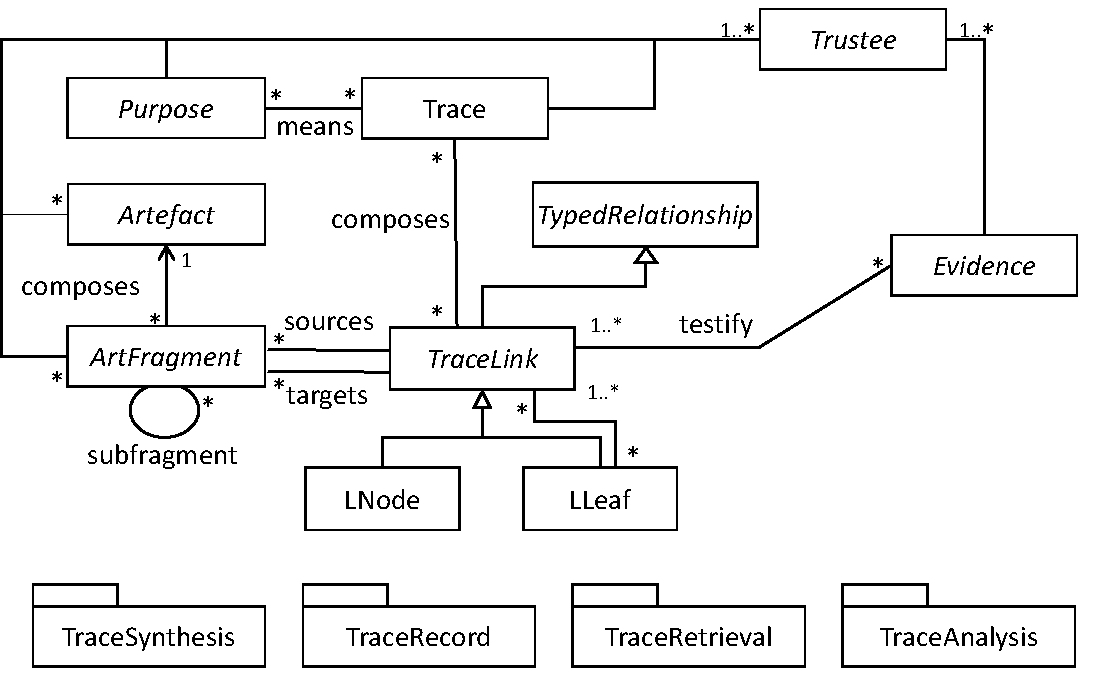
\includegraphics[width=.6\linewidth]{images/metamodel}
	\caption{Indicative metamodel.}
	\label{fig:metamodel}
\end{figure}

As a first contribution of this work, we propose a generic traceability metamodel that helps to formalize better the relationships between the terms described above. This metamodel will also be used through out the paper to discuss and compare traceability approaches, together with the feature model presented later on. At its core, the metamodel comprises a generic representation of tracing artefacts: the links composing a trace, their respective evidences and trustees, and the decomposition of trace and system elements. As pictured in \Fig{fig:metamodel}, a \texttt{trace} is composed of a set of arborescent \texttt{links}. Taken in its broader sense, a trace is a forest of links that connects one or more source \texttt{fragment} to one or more target fragment. Links are \texttt{typed relationships}. This typing allow for a semantic definition specific to the targeted application domain. %For example, a code generator will connect configuration files with the executable of the generator, themselves connected to the generated source code. There is not necessarily a need for all links to be represented but it might be of great help to have a structure robust enough to decide which ones of these links must be represented for analysis. 
Each link is associated with an \texttt{evidence} that testifies the level of confidence of that link. The reliability is affected whether the link has been created manually or inferred automatically, if there is a rule that assess if the link is still valid or not, if it is not deprecated, and so forth and so on. A link refers to fragments of artefacts. These fragments are decomposition of artefacts that can be decomposed as well. Since traceability is strongly advised for validation and certification of safety intensive software systems, the relation between software or trace artefact and their (human) \texttt{trustee} must also be considered explicitly.




%\section{Research questions}\label{sec:rqs}

Beyond the overall goal of analyzing the state of the art in traceability research in software/systems engineering and identifying its open research challenges, we are especially interested in the following subtopics that will be the main focus of our analysis when evaluating the papers resulting from the survey.

\subsection{RQ1: How are traces represented?}
\label{sec:rq1}
We are interested in knowing what languages are used to represent traces and how expressive they are. E.g., is it possible to define types of traces? And use them to link clusters of artefacts (or just individual elements)? Can we express the confidence we have in those traces?

\subsection{RQ2: How are traces identified?}
\label{sec:rq2}
Do traces need to be manually created or can they be derived from existing information? If so, what methods can be used for such derivation? These are some of the topics we would like to answer in this RQ.

\subsection{RQ3: What tool support is available to manage and apply traces?}
\label{sec:rq3}
Finally we want to draw a general map of the techniques that traceability approaches use to store and maintain trace artefacts of quality.

\subsection{Survey method} \label{sec:survey}

In this section we depict the methodology we followed to collect papers related to traceability with a peculiar scrutiny on works aiming at modeling/representing traceability information and purposes.


%\subsection{Publication selection process}
\begin{figure}[h]
	\centering
	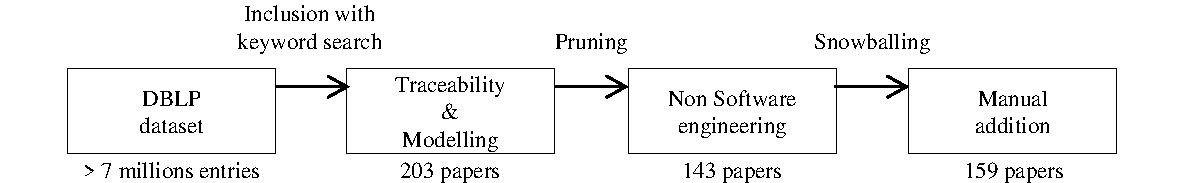
\includegraphics[width=.9\linewidth]{images/survey-process}
	\caption{Process of the survey on traceability and modeling. }
	\label{fig:surveyprocess}
\end{figure}
%\begin{figure}[h]
%	\centering
%	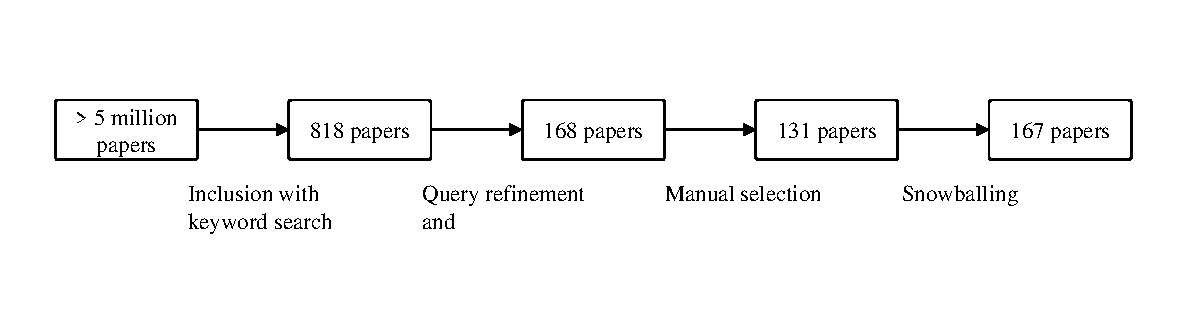
\includegraphics[width=.9\linewidth]{images/survey-process2}
%	\caption{process of the survey on traceability and modelling. }
%	\label{fig:surveyprocess}
%\end{figure}
The approach selection process was conducted in three main steps illustrated in \Fig{fig:surveyprocess}. First, we started selecting approaches based on our own experience about working on traceability during the last past years together with recent meta-studies on the topic, \textit{e.g.,}~\cite{Gotel2012,antoniol2017-traceability-grand-challenges,clelandhuang2014-traceability-trends-and-futurte-direction,guo2017-semantically-enhanced-tracebility-deep-learning}. This very first selection contained a dozen distinct studies we were personally aware of.  

Then, to complement our knowledge and explore the maximum of published work on traceability, we decided to mine bibliographic data sources following the literature review process established by Kitchenham and Charters~\cite{kitchenham2008}.
Finally, we pruned the resulting selection to remove papers not related to our topic.


\subsubsection{Data source and search strategy}
We used DBLP (2020-07-01~\cite{dblp}) as our core electronic database to search for primary studies on traceability.
To avoid missing possibly relevant approaches, we decided not to put a specific period constraint for the search, but we limited the scope of the search to paper of five pages or more to avoid posters, tool demos and other types of short papers.
Based on the topic of this survey, we defined the terms of the search query according to the recommendations of Kitchenham and Charters~\cite{kitchenham2008}. 
As we are looking for papers proposing traceability techniques for software engineering we first considered the terms "trace" and "tracing" together with the seminal spelling "model" referring to modeling, as well as model-based variations. The idea of this first attempt was to include as many proposals as possible by using these generic model-based terms that should be part of any traceability work (as both, traces must be represented, typically as some kind of model, and many traceability approaches use models as source or target of the traces).

Nevertheless, this resulted in too large a number of results with 1100 papers matching the query. Potential papers, at first sight, consisted in a vast majority of false positives. Indeed, "Model" is used in too many fields, "traces" as well, and papers related to software engineering were scarce.
%Since we are not necessarily interested in publications figuring concrete applications of traceability but rather modelling (in a broad sens) work on traceability, we narrowed the scrutiny of the search to work on traceability (modelling tracing) only and we refined once more our query with "traceability", "traces", and "tracer" instead of "trace" for a selection of 771 papers.
Therefore, we refine the query including keywords more akin to modeling and software engineering, focusing more on papers mentioning traceability and not just trace and "modeling" (and its variations and related concepts: "language", "DSL", "transformation", "MDA", "MDD"). This refinement brought down the selection of 203 papers. 

Here is the exact query we applied:
\begin{verbatim}
	.*(([Tt]rac(eability|ing))|([Tt]race[rs])).* AND
	.*(([Mm]odel[- ])(([Dd]riven)|([Bb]ased))|MD[DAE]|Model[l]ing|
	[Tt]ransformation|DSL|[Ll]anguage).*
\end{verbatim}


\subsubsection{Pruning}
In what follows (and as proposed by Kitchenham and Charters~\cite{kitchenham2008}), we describe the used inclusion and exclusion
criteria. We further explain how we applied these criteria on the previous set of papers. 

\textit{Inclusion criteria}
\begin{enumerate}
	\item the work is a software engineering approach
	\item the paper is about tracing software engineering
	\item traceability is the main concern
\end{enumerate}

\textit{Exclusion criteria}
\begin{enumerate}
	\item the paper is not a primary study
	\item paper is not a white paper
\end{enumerate}

Before we applied these criteria on the potential papers fetched by our query, we removed automatically papers of less than 5 pages long.
We then extracted automatically papers whose titles mention "biology", "education", "kinetics", "logistics", "physiology", "physics", "neuroscience", "agriculture", and "food" which seem to appear each in a couple of selected papers. This helped in the application of the exclusion criteria. We manually examined the 183 papers left and excluded 60 papers that did not fulfilled the criteria or were duplicates.
% for a remaining total of 123.

\subsubsection{Snowballing}
Following the application of our methodology, we wanted to double-check that we did not miss any potentially relevant approach. Indeed, some papers could have been missed during the search process for different reasons. For instance, some workshop papers are only indexed by ACM and some other papers have not yet been indexed by DBLP. Furthermore, some papers are not actually using the term "trace" or similar in the title (e.g., if they present so-called composition or extension approaches sometimes used as traceability mechanism). Finally, we added papers we found following the selected papers references and added papers from a specific event on traceability, the ECMFA workshop on traceability (\ie ECMFA-TW). The final result of the overall process (including this last snowballing phase) presented 159 papers. Among them, there are 41 articles, 82 in proceedings, and 36 workshop reports (see Table \ref{tab:classification-tm}).
\Fig{fig:publicationyears-tm} shows the chronological distribution of this selection of publications.


\begin{figure}[h]
	\centering
	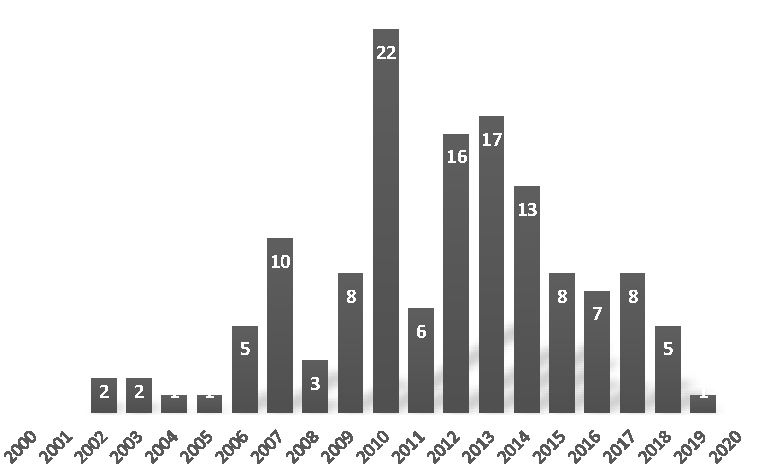
\includegraphics[width=.6\linewidth]{images/publicationyears-tm}
	\caption{Papers selected related to traceability and modeling. }
	\label{fig:publicationyears-tm}	
\end{figure}

\begin{table}[h]
\centering
	\begin{tabular}{|ll|}
		\hline
		\multicolumn{2}{|l|}{\textbf{Publication type}}  \\ \hline
		\multicolumn{1}{|l}{Journal}          & 41       \\ \hline
		\multicolumn{1}{|l}{Conference}       & 82       \\ \hline
		\multicolumn{1}{|l}{Workshop}         & 36       \\ \hline
	\end{tabular}
	\caption{Publication types of the selected papers.}
	\label{tab:classification-tm}
\end{table}



\subsubsection{Threads to validity in the selection process}
We acknowledge limitations in the execution of our survey method. 
First, we only used DBLP as a source database. Yet, it is recognized as a {representative} electronic database for scientific publications on software engineering and already contain more than five millions publications from more than two millions authors.
Setting the limit based on the number of pages alone to elude short papers is another threat to validity. Yet, it is a reproducible practice that limits the number of papers to analyse and thus helps concentrate on the topic rather than the engineering of the survey. 
Then, the vocabulary related to traceability is scattered among various fields of application with their respective nuances. We mitigate the risk of missing papers with a broad query and we remind the reader that, in this survey, we want to target papers explicitly mentioning traceability -- and doing so, working on the emergence of a search field in itself. 

%\subsection{General trends in traceability and modelling}\label{sec:trendsTM}
%The results of the survey are manifold. First, they explicit the dual nature of traceability approaches where the frontier between augmenting traceability and augmenting a software task with traceability is often very thin. 
%\ugh{(rq1)} We found that traceability is specifically adapted to model-based environment, which various levels of abstraction  allows rich representations of trace artefacts~\cite{santiago2013traceability-in-MDE}. MDE automated tasks are moreover prone to generate traces during their execution - including the execution of higher-order transformations supporting co-evolution between modelling artefacts~\cite{la_Fosse_2018}. 
%\ugh{(rq2)}Then, we found evidences of the penetrating importance of machine learning techniques to bridge the semantic gap that separates natural language document and coded elements of a software system. 
%\ugh{(rq3)}Finally, we found that traceability augments the automation potential of many tasks at every phase of the lifecycle and a raw map of the knowledge area covered by traceability approaches emerges.
%We give details on these different points in the next sub-sections.

%\textbf{Insert some \textbf{statistical distribution} (MM/Meta/concrete application | Modelling traceability vs Tracing modelling | identification of traces | Req. vs other | unstructured text vs others (code, or design model))...}
%63 papers are related to requirement traceability (tracing requirements to other software artefacts).
%8 Meta studies
%76 approaches presenting a language or a framework, and 41 explicitly describing a metamodel.
%22 approaches to trace identification with IR techniques
%22 target source code
%51 target model-level artefacts maintenance and understanding
%






%\section{Knowledge area (breakdown)}\label{sec:ka}
We found in our survey that the study of software traceability breaks down into three subcategories. 



\section{A feature model to characterize software traceability}\label{sec:fm}
%\ugh{This is paraphrase from SDI speech-to-text}
This section presents our conceptualization of traceability by means of a feature model describing the traceability features and dimensions found in the analysis of the literature conducted in the previous section. Our feature model groups them by similarity and provides additional descriptions on the most important aspects of each one, \textit{e.g.}, different existing alternative implementation of the same feature and/or the most/the least studied ones in each group.  

%we present a classification that cover components needed for traceability, based on a set of common characteristics found in selected studies from previous section. Considering the lack of a consolidated terminology in the literature, we have extracted the characteristics and grouped them by similarity. Next, a generic nomenclature was assigned for each group, so that similar characteristics in a group are represented in an unified way. 

Next subsections provide some background on feature modeling and then zoom in each of the three main dimensions of traceability: trace representation, trace identification, and trace management. These dimensions are depicted in \Fig{fig:fm:definition}, \Fig{fig:fm:identification}, and \Fig{fig:fm:management}, respectively. %The feature model was created focusing on the identification of the prominent or distinctive features, i.e., attributes of a system that directly affect end-users’ decisions. 

%Based on the analysis of the papers selected in the previous section, we propose a feature model for software traceability. 
%Our first finding is that the knowledge area of software traceability breaks down into three sub-areas. 
%For each of them, together with a more detailed explanation, we will present a feature model that summarizes the broad set of dimensions that must be considered when describing traceability proposals. 

%The first sub-area targets concerns directly related to trace definition and representation. \Sect{sec:fm:def} relates the associated techniques and distinguishes what kind of languages are used to represent traces and how expressive they are. E.g., is it possible to define types of traces? And use them to link clusters of artefacts (or just individual elements)? Can we express the confidence we have in those traces?  
%In the second sub-area, the means of identifying and recording traces are under scrutiny and differentiates configurations depending if traces need to be manually created or if they can be derived from existing information. If so, what methods can be used for such derivation? These are some of the topics related to trace identification that we would like to disentangle in our feature model in \Sect{sec:fm:identification}.
%Finally, the third sub-area distinguishes the techniques implemented to assist the storage and maintenance of quality traces. 

\subsection{Introduction to feature modelling}
A feature model leverages features as the abstraction mechanism to reason about product variability. It is a hierarchically arranged set of features, where relationships between a parent feature and its child features may be categorized as: \textit{and} – all sub-features must be selected, \textit{alternative} - only one subfeature can be selected, \textit{inclusive or} – one or more can be selected, \textit{mandatory} - features that are required, and \textit{optional} - features that are optional~\cite{kang1998-FeatureModel}.  Each feature represents an increment in product functionality. 

Feature modeling is a technique that has been intensively used for documenting the points of variability in a software product line, how the points of variability constraint one another, and what constitutes a complete configuration of the system. 
%This seminal work from Kang \textit{et al.} has been cited thousand times. To complement feature-modeling tooling, researchers contributed hundreds of feature-model analyses, refactorings and management techniques, as well as automated synthesis techniques. Feature modeling is supported by major product-line engineering tools~\cite{nesic2019-principles-of-FM}. 
But beyond product lines, feature model are also more and more used to shed light on complex domains by representing the core concerns and variation points in a complex ecosystems (\textit{e.g.}, \cite{DBLP:journals/sosym/BruneliereBCW19}), as we do in this paper.

%It can capture different types of variability, ranging from requirements variability to implementation variability. It can also allow for automated generation and verification of complex systems~\cite{metzger2007-feature-model-check}. 


\subsection{Trace definition and representation}
\label{sec:fm:def}
\begin{figure*}[h]
	\centering
	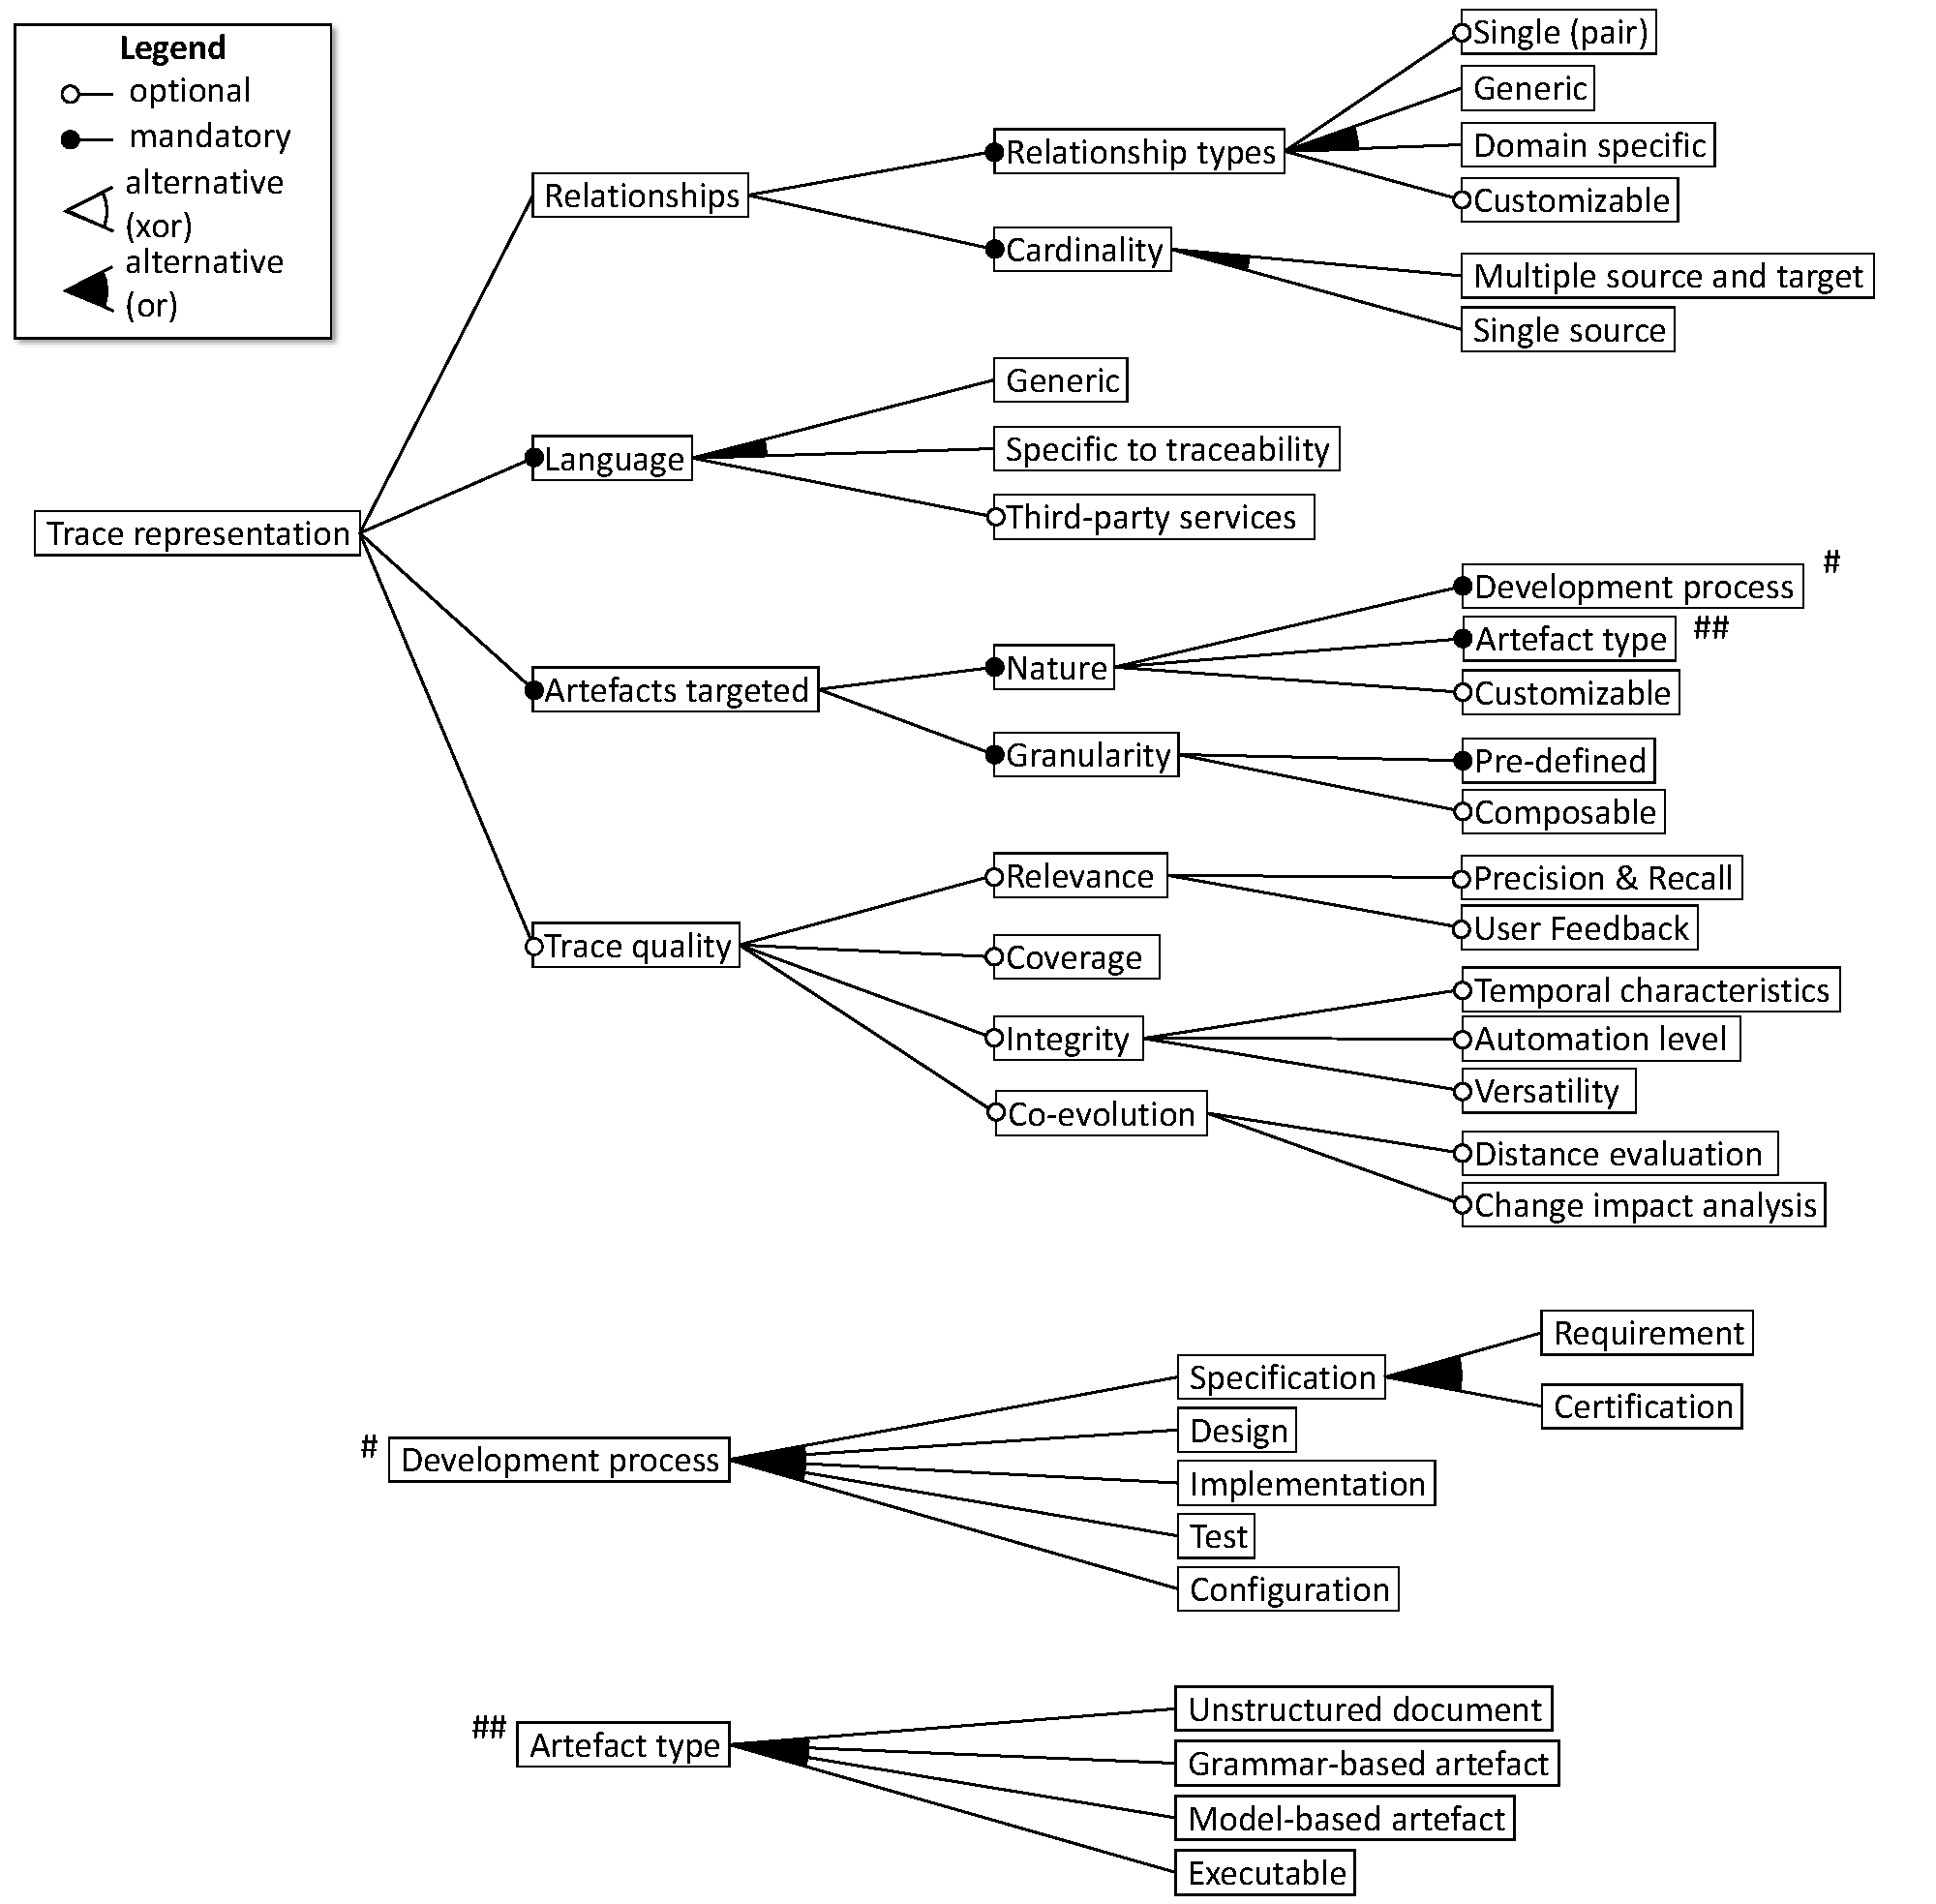
\includegraphics[width=.8\linewidth]{images/fm-definition}
	\caption{Features related to the representation of a trace.}
	\label{fig:fm:definition}
\end{figure*}

%As discussed in the terminology section, there is no common representation or standard for traceability. Instead, we find a plethora of applications of traceability in specific domains such as program understanding, with approaches facilitating the localisation of features~\cite{seiler2019-comparing-trac-through-IR-Commits-Logs} and bugs~\cite{ko2008-whyline-debugging}. Traceability eases software decomposition into relevant partitions~\cite{laghouaouta2017-model-composition-tracaebility} or slices~\cite{nejat2012-traceability-sysml-safety-certification}, it eases software reuse ~\cite{tinnes2019-improving-art-reuse-with-traceability} and provides support for the general explainability of the software process and product~\cite{wohlrab2020-traceability-organization-process-culture}. 
%Traces are used to help gath%er evidences for certification. 

All approaches must discuss their representation of trace artefacts even if they can differ already based on the type of traces they consider and their foreseen application. Representations are so diverse that our survey selected more than 80 papers mentioning their own distinct definitions with 20 metamodels effectively depicted in those papers.
Some researchers present generic graph-based representations ~\cite{schwarz2010-graph-based-traceability,grammel2012-model-matching-for-traceability-in-MDE} while others focus on representations much more specific to a concrete application like this metamodel for %  the verification and validation of software artefacts~\cite{Dubois_2010,vonknethen2002-change-oriented-req-traceability-evolution-of-embedded-systems} and traceability artefacts~\cite{rempl2014-conformance-of-traceability-to-guidelines} ; others target the maintenance of software systems with representations for 
change impact analysis~\cite{goknil2014-change-impact-analysis-for-requirement-metamodel} or multi-model consistency~\cite{Szabo_2013}.
%\eb{So many perspectives shall provide enough details for a standard, or at least a common understanding (cf our metamodel?).}

\Fig{fig:fm:definition} shows the hierarchy of features related to the definition and the representation of trace artefacts. A peculiar focus is put on the typing of the traces relationships. Typing relationships is important to add semantics to the trace so that the engineer can know not only what are the linked artefacts but also why they are linked. As such, it facilitates the  application of traceability solutions to specific domains. We also detail the genericity of the language, the artefacts covered by the traceability proposal and the possibility to annotate traces with quality properties.

We would like to remark the contribution of model-based approaches for traceability in this subsection. The use of MDE tooling such as ATL~\cite{Santiago_2013,Jim_nez_2013}, or the Eclipse Modeling Framework (EMF) allows the automated generation of traceability information as a side effect of executing operations~\cite{galvao2007-survey-traceability-in-MDE,winkler2010-survey-traceability-and-MDE}. The modeling community has proposed  metamodels for end-to-end traceability~\cite{heisig2019-generic-traceability-metamodel-end-to-end-capra,Haidrar_2016}, as well as metamodels specific to engineering domain such as model transformation~\cite{Jim_nez_2013,anquetil2010-model-driven-tracea-for-SPL,vara2014-traceability-in-MDD-MTransfo,bonde2006-different-levels-of-abstraction} or software product line~\cite{Jim_nez_2013,vara2014-traceability-in-MDD-MTransfo}. 
%The Requirement Interchange Format (ReqIF) is an attempt to standardise requirement tracing in the EMF community~\cite{Graf_2012}.
%Yet, industry has not standardised on EMF -- they use a wide variety of technologies for modeling, and some of it does not conform to the usual notions of modeling technology: they may not have explicit metamodels.
Paige \textit{et al.} call for more flexible modeling where models of different formats are associated to each others' with annotations that allow automated bond or dependency inference between both application and engineering domains~\cite{seiler2019-comparing-trac-through-IR-Commits-Logs,paige2017-changing-mde}.

\subsubsection{Artefacts targeted} 
In relation to the artefacts targeted by traceability purposes we distinguish between the nature of the artefact and its granularity as both dimensions are important and used in the literature. 

For the nature aspect, on the one hand, investigations differ on the development phase they target. Linking requirement specifications to design and code level predominate in the literature with more than 50\% of the papers in the survey addressing requirement traceability. Other phases such as test and verification are targeted as well but in a lesser proportion. 
On the other hand, the type of the artefacts is important to deduce the level of potential generalization to other phases of the software lifecycle. Papers focus on four different types: unstructured document, structured as grammar-, and model-based artefacts, and binaries.

With regard to the granularity of the artefacts targeted, \textit{i.e.}, their level of decomposition, some approaches go for a customizable granularity to adapt to artefact hierarchies while others  focus on specific types of artefacts (\textit{e.g.,} to concentrate their work on specific optimizations of trace identification).
%Rosenkranz \textit{et al.} attempt to trace communication in the development process and show that quality evaluation of requirements is an important factor to further evaluate and trace their impact~\cite{Rosenkranz_2013}. 

\subsubsection{Language} 
Languages specific to traceability provide the ability to represent trace artefacts with increased relevance and accuracy. Yet, they often suffer the limitation to be built \textit{ad hoc} and lack a significant power of reusability other domains and risk of ending up reinventing the wheel. Among these domain-specific languages for traceability, some authors attempt a generic definition of traceability~\cite{heisig2019-generic-traceability-metamodel-end-to-end-capra,azevedo2019-traceability-metamodel-and-reference-model} while others provide a language specific to a single domain, \textit{e.g.}, traceability for software product lines~\cite{anquetil2010-model-driven-tracea-for-SPL}.

We found few studies interested in the use of general-purpose software language for traceability - even though this would be appealing to industrial partners interested in instrumenting their legacy systems code with traceability information to facilitate future evolutions or migrations~\cite{nejat2012-traceability-sysml-safety-certification}. 
Another type of general languages for traceabiity could involve representing traces in spreadsheets, text files, or databases. This shows better learning curves than using a domain specific language at the cost of a cognitive gap between software engineers and domain experts. As an unfortunate consequence, "the maintenance costs turns out to grow accordingly [to the usability of generic representations] and team members fail to keep the trace artefacts up-to-date"~\cite{clelandhuang2007bestPracticeForAutomatedTraceability}.

A potential sweet spot could be to ``plug'' traceability concerns on top of other languages like SysML ~\cite{nejat2012-traceability-sysml-safety-certification} to benefit from an existing language structure while keeping most of the benefits of using a DSL. 

\subsubsection{Relationship types} 
As many authors have demonstrated, offering the ability to the user to define personalized types of relations between the artefacts of a system fosters the comprehensibility of the traces produced~\cite{olive2002-representation-of-generic-relationship-types-in-modeling}. We distinguish between approaches offering predefined types, most often relating to the field of software engineering (implements, inherits, uses, executes ...) and approaches allowing custom typing. %The formers allow increased monitoring and user-friendliness \textit{for IT experts}. They are not very attractive to \textit{experts in other sectors}. 
%Publications focusing on trace identification rarely consider other types of artefacts. They rather focus on the peculiar pair their optimisation targets.
%Allowing users to define the types of relationships specific to their area of expertise helps to fill the gap between the design and the use of tracing functionalities~\. %The communication gap that lies between respective communities also benefits~\cite{wohlrab2020-traceability-organization-process-culture}.

Obviously a fixed typing facilitates the analysis of the traces as the potential set of semantics and interpretations are fixed while offering domain-specific types increases the usability and comprehensibility of the approach. As an example, SysML v2 is offering a more powerful mechanism to define links between artefacts. Compared to the previous SysML version (where we had a sole dependency-like mechanism) we now have the ``Connection'' concept that is customizable and that could be regarded as a good equivalent for our trace link concept. 

The literature shows also a distinction between approaches considering relationships with multiple sources and targets and relationships allowing only a single source.  

\subsubsection{Trace quality} 
In most of the papers we studied, quality aspects were barely mentioned. It seems quality of the generated traces is not a major concern, or at least storing and annotating the traces with such information is not.

Yet, a few studies mention coverage and integrity.
The coverage of a set of execution traces is used in approaches for software testing~\cite{gannous2019-Certification-into-Model-based-Testing-for-Safety-Critical-Systems}. Coverage is also used by Rath \textit{et al.} who address the problem of missing links between commits and issues with a classifier they train on textual commit information to identify missing links between issues and commits (\ie a lack in the coverage indicates such missing links)~\cite{rath2018-guo-augmenting-incomplete-traces}. Integrity of traces is addressed in work on model transformation where co-evolution figures an automatic verification of their coherence with other (versatile) software artefacts~\cite{Szabo_2013,slotosch2018-Modeling-and-Certification-of-MDD-Processes}. 
The co-evolution of traces implies measuring distances between artefacts (syntactic, cognitive, geographic, cultural...)~\cite{bjarnasson20016-theory-of-distances-in-SE}.  It also refers to the analysis of the changes of the system that impact traceability artefacts~\cite{goknil2014-change-impact-analysis-for-requirement-metamodel,vonknethen2002-change-oriented-req-traceability-evolution-of-embedded-systems}. In our survey, nine papers address artefacts co-evolution and 17 tackle model transformation limitations. These latter are a valuable tool to automate co-evolution tasks. 
In the many studies focusing on the optimization of link identification, the quality of the results is mainly evaluated with precision and recall measurements. Few researchers include a user feedback~\cite{borg2014-SmS-IR-for-traceability}.

%All in all, these interesting findings are a minority and a need to understand clearly the purpose of trace-based approaches remains prominent. 
A few publications relate the quality of their work to the computation of aggregated values, evaluated against company (or project specific) thresholds~\cite{Bunder_2017_query-for-quality}. They make use of rules to automate the computation of customizable analyses and show that query, metric and rules are a powerful combination to measure the productivity of new initiatives.

\subsection{Trace identification}
\label{sec:fm:identification}
\begin{figure*}[h]
	\centering
	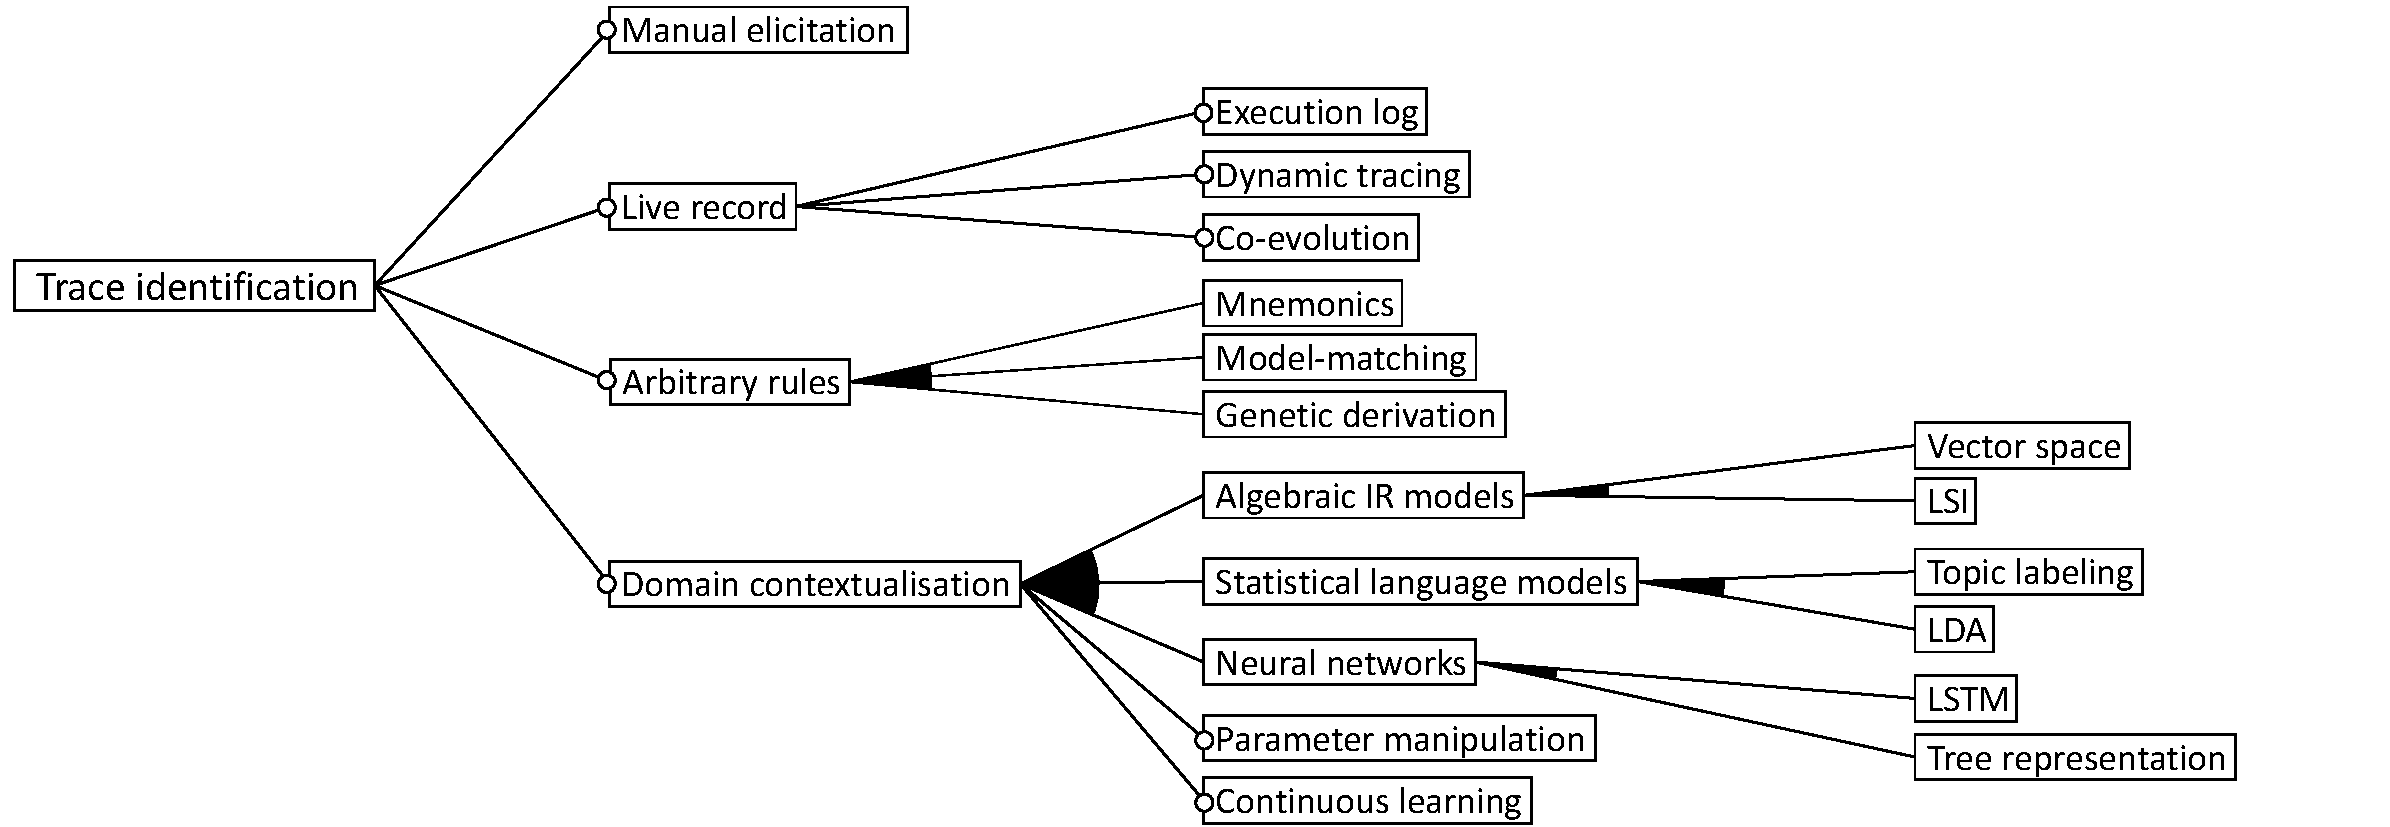
\includegraphics[width=.8\linewidth]{images/fm-identification}
	\caption{Features related to the identification of trace links}
	\label{fig:fm:identification}
\end{figure*}

%Many publications tackle the difficulty to automate the identification of trace links and introduce approaches based on the application of natural language processing techniques. 
\Fig{fig:fm:identification} shows the hierarchy of features related to the identification of traces with four main possible categories: 
the manual elicitation of traces, 
their live record during execution and evolution,
rule-based alternatives to assist the user with automation potential, 
and AI-augmented identification with domain contextualization.


\subsubsection{Manual elicitation} 
Manual elicitation makes possible to create traces in an \textit{ad hoc} manner. As an example, one of our industrial partner chose to hire a developer to elicit trace links necessary for a certification commitment. This was chosen rather than a (semi-)automated approach as they were not convinced the effort of augmenting an existing tool would pay off for that specific project. 

\subsubsection{Recording instrumentation} 
Teams can instrument the {live record} of traces during the execution and the evolution of software artefacts. This way traces recording the system changes are a side-effect of those same changes. There are initiatives to instrument existing languages such as ATL with rich log generation~\cite{Santiago_2013,la_Fosse_2018}, while others consider trace record an aspect that can be weaved with current existing languages~\cite{Pfeiffer_2014,Santiago_2013}. Ziegenhagen \textit{et al.} mix execution traces with metadatas~\cite{ziegenhagen2020-expanding-tracea-with-dynamic-tracing-data}, and use developer interaction records~\cite{ziegenhagen2019-developer-tool-interaction} to enrich existing traceability artefact.

Model transformations are considered the hearth and soul of software modeling and, consequently, numerous studies attempt to enrich trace generation during transformation execution~\cite{vara2014-traceability-in-MDD-MTransfo,Saada_2013,la_Fosse_2018}. This ubiquitous integration (see \Fig{fig:fm:management}, bottom branch) allows a semantically rich tracing of target and source artefacts~\cite{paige2011-traces-in-moel-driven-engineering}. Unfortunately, this option can only be applied when we are building the system, not when the system is already in place.

\subsubsection{Arbitrary rules} 
%Once a system is in place, the links that one might want to use (for locating features, increasing code understanding, and reducing perpetual maintenance effort) can be partly recovered automatically. Indeed, the knowledge that programmers process when writing the code is often captured by the mnemonics for identifiers~\cite{antoniol2002-tracing-code-documentation-links}. The analysis of these mnemonic means allows the constitution of linkage rules between software artefacts. The example of the similarity between Java classes file names and their respective binaries is obvious. 
Once a system is in place, teams can identify rules that help retrieve and maintain traceability relations~\cite{mader2008-rule-based-maintenance-post-requirements-traceability,spanoudakis2004-rule-based-generation-of-req-traceability-relations}.
Antoniol \textit{et al.} use the mnemonics for identifiers to establish trace identification rules~\cite{antoniol2002-tracing-code-documentation-links}.
At the model level, Grammel \textit{et al.} use a graph-based model matching technique to exploit metamodel matching techniques for the generation of trace links for arbitrary source and target models~\cite{grammel2012-model-matching-for-traceability-in-MDE}, and Saada \textit{et al.} recover  execution traces of model transformation using genetic algorithms~\cite{Saada_2013}.


\subsubsection{Domain contextualisation} 
Borillo \textit{et al.} published an article on the use of information retrieval techniques for linguistics applied to spatial software engineering~\cite{borillo1992-linguistic-engineering-to-spacial-SE}. This precursor work opened the box for AI-augmented traceability where machine learning algorithms help extract knowledge specific to the application domain. This is specially useful when the source (or target) of the trace link is an unstructured document or when such document is key to infer traces among other artefacts.

Researchers first extracted word vectors from natural language. Vectors intend to take account of the neighbouring words a term may relate to in the application domain~\cite{delucia2012-information-retrieval-for-traceability}. This effort made the identification of bonds between requirement specifications and other artefacts possible with a gradually improving precision. Since then, many other information retrieval techniques for natural language processing were applied with success~\cite{arunthavanathan2016-traceability-with-NLP}. Studies on domain contextualization are separated into three subgroups according to the type of tools used (algebraic information retrieval models, statistical language models, and neural networks).  For example, Florez \textit{et al.} derive fine grained requirement to source code links~\cite{florez2019-finegrained-req2code}, Rath \textit{et al.} complete missing links between commits and issues~\cite{rath2018-guo-augmenting-incomplete-traces}, Marcus \textit{et al.} identify links between documentation and source code~\cite{marcus2003-latent-semantic-indexing-for-traceability-LSI}. An interesting publication from Poshyvanyk \textit{et al.} shows that mixing expertise both in information retrieval techniques and engineering domains gives far better results than when taken separately~\cite{poshyvanyk2007}.

Today, domain contextualization by means of machine learning for topic modeling, word embedding, and more generally knowledge extraction from unorganized text documents is the most popular traceability feature~\cite{guo2017-semantically-enhanced-tracebility-deep-learning,wohlrab2020-traceability-organization-process-culture}. We found 22 approaches dedicated to this topic alone in our survey. 

Teams are also using genetic algorithms here, not to recover traces themselves but to cope with the variety of algorithms and parameters these approaches use~\cite{marcen2020-req2model-with-EA-ranking-train-system,panichella2013-genetic-programming-for-effective-topic-modeling}, and structural information to foster methodologies interweaving~\cite{panichella2013-using-structural-information-to-improve-IR-traceability}. Unfortunately, a common critique rose against these positive results. 
Too many teams compete with each others to accomplish a better precision and recall when there is no standard to the effective quantification of traces artefacts into such variables. Too few attempt at qualifying the overall relation between these measurement and the effective impact on software development~\cite{clelandhuang2014-traceability-trends-and-futurte-direction}. 

In that regard, Shin \textit{et al.} propose guidelines for benchmarking automated traceability techniques. Their evaluation (of 24 approaches) shows that methods of evaluation (when they are used appropriately) sometimes are not suitable to other application domains and that the variation in evaluation results across project is not investigated~\cite{shin2015-guidelines-benchmark-auto-traceability}. This corroborate Borg \textit{et al.} who, in a systematic literature mapping on information retrieval approaches to traceability, notice that there are no empirical evidence that any IR model outperforms another model consistently~\cite{borg2014-SmS-IR-for-traceability}. The ability to continuously improve the learning process is mentioned in the literature but we found no evidence of its application. 

\subsection{Trace management}
\label{sec:fm:toolsupport}
\begin{figure*}[h]
	\centering
	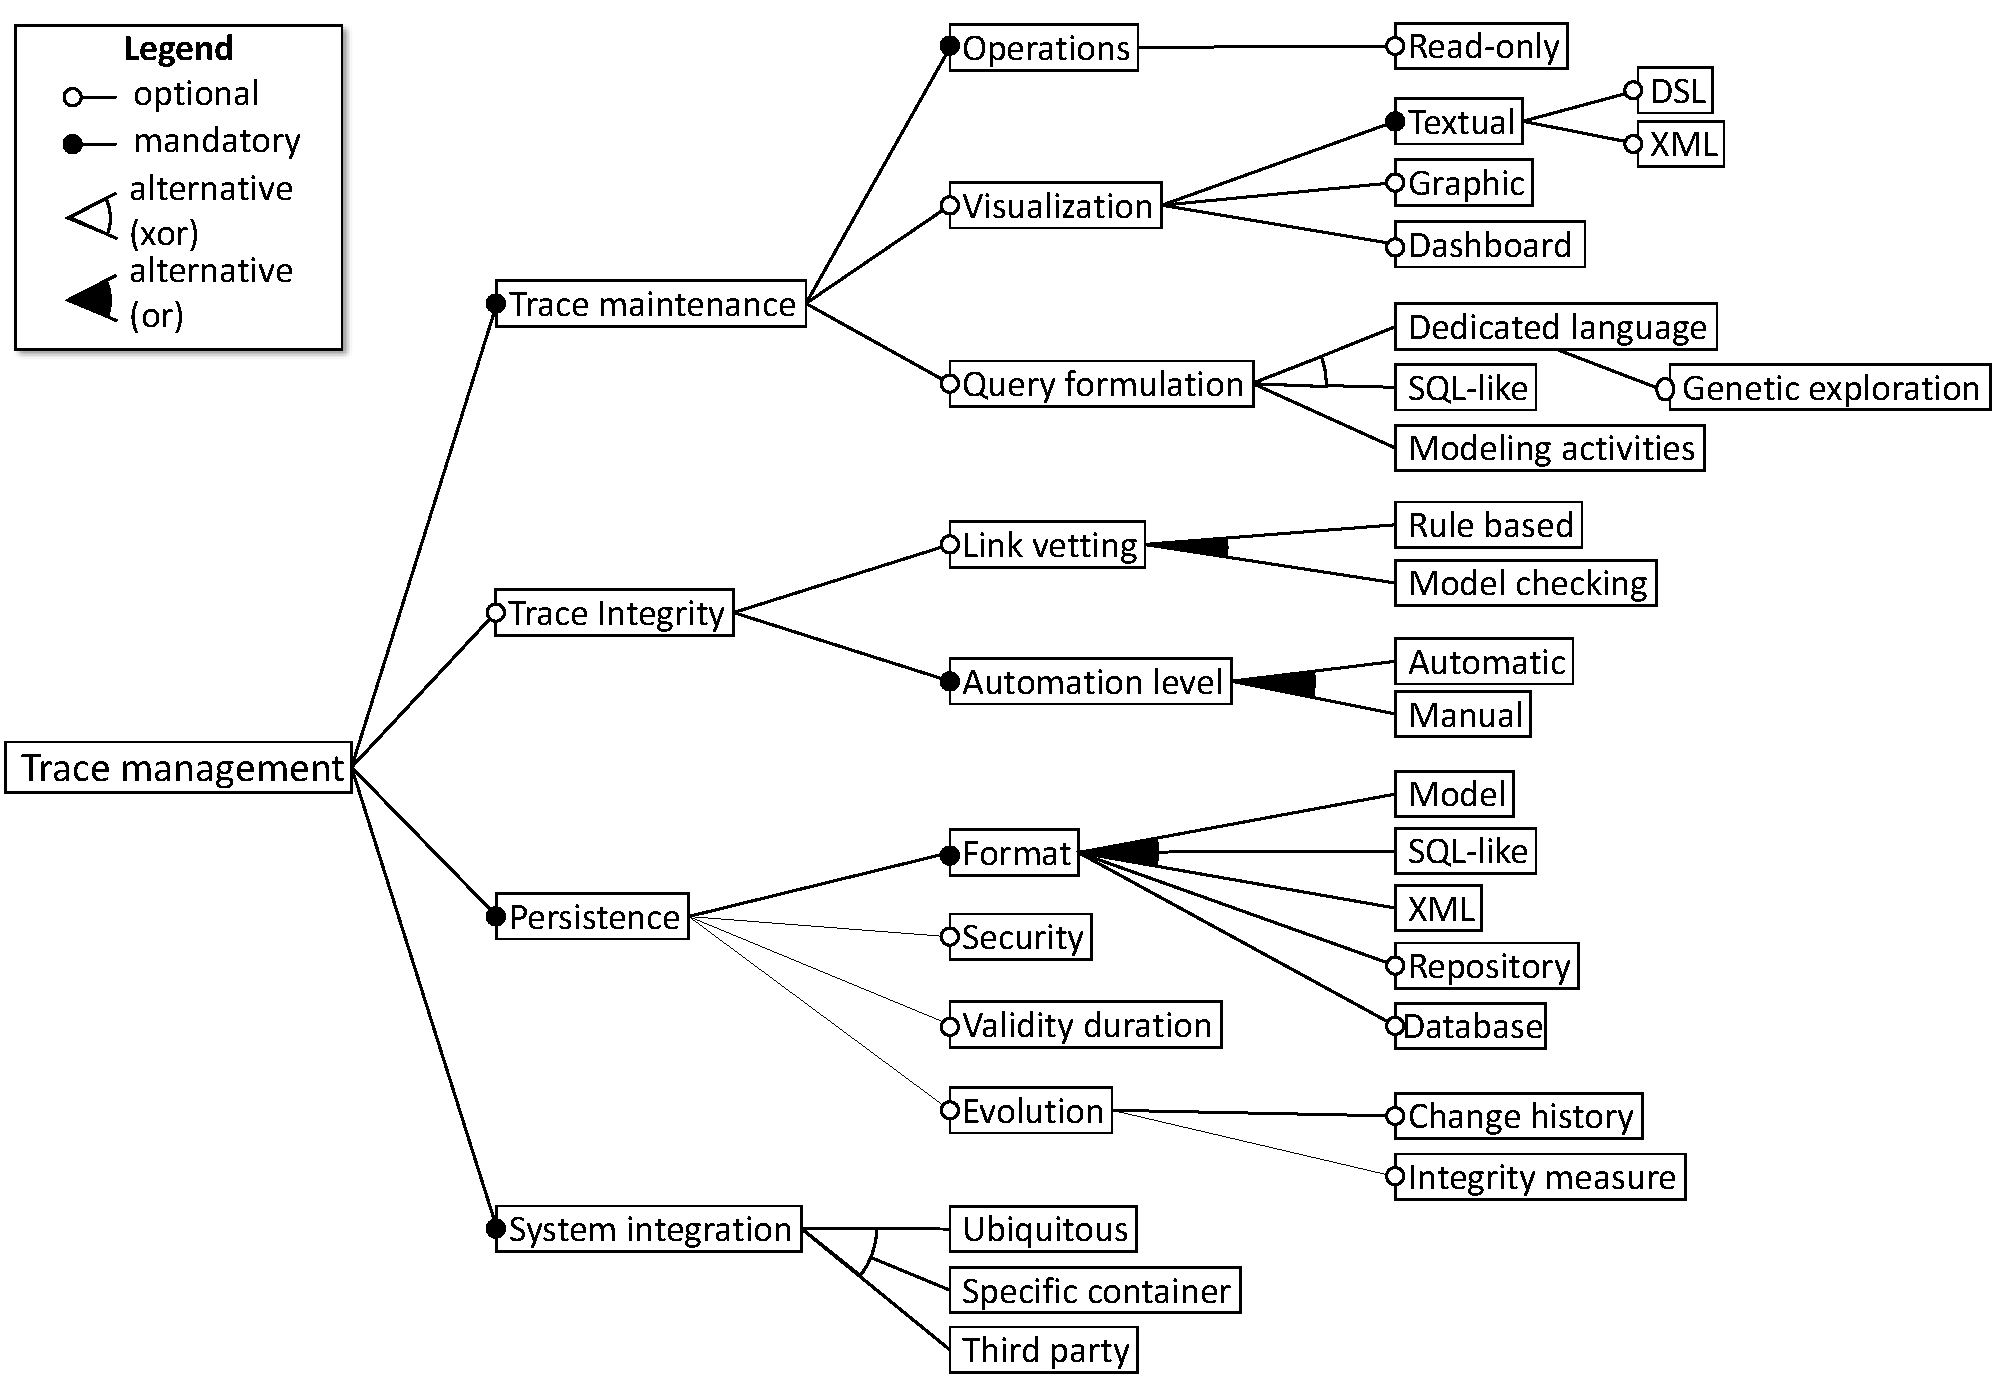
\includegraphics[width=.8\linewidth]{images/fm-toolsupport}
	\caption{Tool support for traceability management.}
	\label{fig:fm:management}
\end{figure*}

\Fig{fig:fm:management} shows the hierarchy of features related to the management of trace artefacts. We distinguish between the actual maintenance of trace artefacts, the evaluation of their integrity, the means of persistence, and the level of integration in running software systems.

\subsubsection{Trace Maintenance} 
Trace links may be affected by changes on the artefacts they are linking to (directly or transitively) and therefore can easily become obsolete. This gradual decay must be seriously taken into account to avoid having to re-elicit traces every time they need to be analyzed. A manual maintenance is not always impossible but not typically feasible in practice due to the amount of information such inspections would involve. % This motivates a serious consideration of automated ways to retrieve and then visualise traces. 
%The vast amount of potential trace links traceability approaches have to handle motivate a serious consideration of automated ways to visualise and retrieve them. 
Co-evolution techniques~\cite{mader2008-rule-based-maintenance-post-requirements-traceability,drivalos2010-state-based-traceability,rahimi2019-Evolving-trace-req2source} attempt to tackle the burden to maintain trace links up-to-date~\cite{seibel2010-dynamic-hierarchical-models-comprehensive-traceability,Bunder_2017_query-for-quality}. 

Beyond being able to manipulate traces, we also need to offer proper ways to visualize and inspect them~\cite{fittkau2013-explorviz-Trace-Visualization}. The use of graphical representations stimulate human perception and the integration of such technique in traceability frameworks is a useful feature to augment user awareness~\cite{heisig2019-generic-traceability-metamodel-end-to-end-capra}.
In parallel, allowing a rich formulation of queries to assist the exploration of existing traces will help to reduce the amount of information users need to navigate through~\cite{Bunder_2017_query-for-quality}.
More precisely, structured text, in the form of metamodel instances or XML sheets allows query-based mining of trace datasets~\cite{dietrich2013-learning-efective-query-transformation-for-enhanced-req-trace-retrieval}. Interaction wise, hyper-text links is a \textit{de facto} standard to browse trace links. Indeed, following links through successive clicks has become almost natural.  Querying depends on the type of representation of traceability artefacts. SQL-like languages benefit from a long history of information mining while dedicated languages offers better legibility. Genetic programming has also permitted the automation of query formulation~\cite{perez2020-genetic-query-reformulation-for-feature-location}. 

%All in all, assisting efficiently end-users in the retrieval, visualization and analysis of traces is not easily granted. Yet, studies on the topic remain scarce in comparison to other concerns. There is still great space for improvement and calls for more work in that direction are redundant through literature studies~\cite{Gotel2012,antoniol2017-traceability-grand-challenges}.

\subsubsection{Trace Integrity} 
To cope with the decay and volatility mentioned above, we need a way to determine the integrity of existing traces. Work on these questions, although called out loudly by literature studies, is scarce in practice~\cite{winkler2010-survey-traceability-and-MDE,antoniol2017-traceability-grand-challenges}. The first option is given with manual annotation or vetting of trace links to inform about their level of reliability. Annotations allow a qualitative and quantitative evaluation~\cite{Buchmann_2015}. This is the case for back-propagation of verification and validation results between design and requirements~\cite{Hegedus_2010}.  

Some approaches enable the definition of invariant rules while manipulating traces or their targets~\cite{Bunder_2017_query-for-quality}. If the invariant is violated, an exception for that trace is automatically generated. For example, we could define a rule that is violated when a change occurs in an artefact targeted by a trace if the corresponding link was identified more than two versions prior to the current version. 

\subsubsection{Trace persistence} 
\ugh{Security?}

Many different storage alternatives exist for traceability artefacts.
An option is to use SQL-like grammar to store and retrieve traces with the power of database tooling, or to use XML documents to represent trace matrix in a transformable format. The industry uses a lot of informal format and link representations often remain implemented in spreadsheets, text files, databases or requirement management tools. These links deteriorate quickly during a project as time pressured team members fail to update them. 
Researchers aiming at a generalizable approach favour model-based representations able to express specifically defined concepts related to traceability (often in a specific domain of application). The burden of maintaining traces coherent is eased in model-based solutions~\cite{clelandhuang2007bestPracticeForAutomatedTraceability}. Elamin \textit{et al.} propose to implement traceability artefact in graph based databases to improve software quality~\cite{elamin2018-repositories-as-graph-databases}.

Another concern lies in the recording of trace evolution. The trace creation should be recorded, with the successive changes that affect it, for evolution analysis. Integrity measures respective to evolution events (\textit{e.g.,} creation, modification...) should be recorded as well to evaluate their evolution during a period of time. Rahimi \textit{et al.} ensure the co-evolution of artefacts and traces~\cite{rahimi2019-Evolving-trace-req2source} using a set of heuristics coupled with refactoring detection and information retrieval to detect changes scenario between contiguous versions of software systems.

\subsubsection{System integration} 
Like most of the MDe approaches, Helming \textit{et al.} use of the same modeling language for both traceability and system artefacts to track changes~\cite{helming2009-traceability-change-awareness}. The conjunct use of EMF and a dedicated traceability metamodel (both written in Ecore) facilitates the integration of traceability features including graphical versions to stimulate human perception and standard analysis of traces in the native (Ecore) environment of the traced system. 

Galvao \textit{et al.} in their seminal work on traceability and MDE call for more loosely coupled traceability support that can integrate external relationship with independent representations (in another, ideally common language)~\cite{galvao2007-survey-traceability-in-MDE} as also elaborated by Azevedo \textit{et al.}~\cite{azevedo2019-traceability-metamodel-and-reference-model}. 




\section{Discussion}\label{sec:discussion}

The feature model is a first step towards the shared understanding of all dimensions involved in a traceability solution. Ideally, a company interested in a certain set of such dimensions could try to create its perfect traceability solution by combining the top solutions for each dimension. But this is not yet a real possibility as those solution would be difficult to combine and, more importantly, several of the features in the feature model do not really have a great solution yet. This section elaborates on this discussion by presenting some open challenges in software traceability research.

\textbf{Common traceability metamodel}. We have counted over 20 different metamodel proposals. Some are solutions to specific problems the authors present as case studies. And these metamodels are rarely reused, if ever. This proliferation is a challenge to make different traceability solutions interoperate. The research community should agree in a unified proposal that facilitates the composability of traceability solutions. We believe Eclipse Capra~\cite{heisig2019-generic-traceability-metamodel-end-to-end-capra}, even though build to address software product line tracing, could provide a solid foundation for this unified metamodel as it already comes with good tool support to build on.\ugh{Precise: for MBSE.} \ugh{Customization and visualization tooling. Generic link definition. External language based on Ecore/XMI.}

\textbf{Complete traceability metamodel}. Following up on the previous point, to agree on a core traceability representation may not seem difficult but it would ignore many of the aspects in the feature model that we believe are key in any non-trivial and industrial traceability application, such as the quality and temporal annotation of traces. A core model with an extension mechanism could be a good compromise here.

\textbf{Security of trace data}. Considering that traceability is a major aspect in certification and other critical applications, it is surprising to see very little interest in security concerns related to trace artefacts. We believe security mechanisms (even simple rule-based access control) for traceability are needed to control who can modify what trace data, given the implication such changes can have. 

\textbf{Library of trace types and semantics}. We already mentioned the importance of having a rich set of types for traces to let engineers express the reasons behind the creation of a given trace. But at the same time, complete freedom makes reusability of analysis techniques difficult. We would like to see a rich yet predefined set of types for traces that could then be imported in new traceability projects.

\textbf{Usefulness of identified traces}. Managing a large number of traces is time consuming. As such, we should make sure every explicit trace is actually useful. So far, algorithms aimed at automatically identifying traces are compared based on standard properties like precision and recall. But they should be evaluated on ``usefulness'': are those traces useful for the end-user? or are just redundant noise? 
%hese questions have been long due and a common conceptualization of the core tracing abilities will be a first step to distinguish between tracing purposes.
%The efficiency of identification is primarily based on the measurement of precision and recall of the algorithms. This is a widely accepted limitation since this quantification does not take into account what the actually identified traces represent for the end user – are they “useful”? And how? These questions have been long due and a common conceptualization of the core tracing abilities will be a first step in that direction. 

\textbf{Verification, validation and testing of traces}. Our ample literature on verification, validation and testing methods for software engineering should be extended to deal with trace data, especially from a temporal perspective, where temporality would depend on pure timestamp values (i.e. how long since the trace was created) and on evolution lag (i.e. how many times the linked artefacts have changed since the trace was created). Reasoning on outdated and potentially incorrect trace data could have strong damaging impacts on the system as a whole. So far, very few approaches target these aspects except for the specific  problem of coevolution in model-driven engineering. 
The ability to justify – with evidences and uncertainty evaluation – the quality and integrity of traces is a prerequisite to robust and reliable traceability. And given the effort required to create traces in the first place, this is important to instill more confidence to practitioners wondering whether creating traces is worthwhile.

\textbf{Traceability as first-class concern in general languages}. Another important step towards the mainstream adoption of traceability in industry is the integration of the common traceability metamodel in popular modeling languages like UML or SysML, in the form of a profile (to be able to directly reuse existing modeling tools available for those languages) or new packages in the respective standards. This way, traceability would become a first-class citizen in software development while still being a rich concept and not just the plain dependency relationship we can use right now in those languages. 

\textbf{Working together with Industry}. Orthogonal to all the others, we (the research community) should aim to have more frequent exchanges with practitioners to better understand why they end up creating traces manually instead of trying to reuse any of the dozens existing solutions covered in our survey. Some reasons have been already hinted in this paper, based on our own experience in industrial projects involving some type of traceability need and based on the survey we have conducted,  but there could be others we are not aware of. Or a different prioritization than the one we have in mind. If we want traceability research to transfer to industry, more and better communication flows should be part of the agenda. 


%Parallel to these facts, we see a strong dichotomy between generalist and specialist investigations. On the one hand, researchers attempt to build generic approaches and tools and gather material for the pooling of knowledge. Heisig \textit{et al.} offer a fit-for-all metamodel based on (and restricted to) Ecore technology~\cite{heisig2019-generic-traceability-metamodel-end-to-end-capra} ; Tekinerdogan \textit{et al.} present a metamodel for tracing across the software life cycle~\cite{tekinerdogan2007-metamodel-for-tracing-concers-accross-life-cycle} ; Keenan \textit{et al.} present a workbench to evaluate traceability approaches~\cite{keenan2012-workbench-for-traceability}). The adoption of these approaches is hampered by inherent design choice (\textit{e.g.,} using Ecore, putting software life cycle as the main factor)

%The most common objective seems to be the identification of traces. The use of AI has helped a lot develop this important feature for end-to-end traceability. Adaptations and optimizations of machine learning techniques to the identification of traces are numerous. Unfortunately, their adoption by industry remains little. This is due in part to the methods adopted by researcher to validate their work. 
% which remain mainly an arbitrary (precision and recall) quantification. 
%Where the shoe pinches is in the ability to evaluate the benefits of increasing the tracing ability of software outside of comparison between techniques. 


%In this regard, the importance of the typing of links and artefacts is unanimous. It is about allowing the user to manipulate the relational elements and their targets in the language of his or her expertise. The granularity of the target artefacts must be adapted to the field of application as well~\cite{clelandhuang2007bestPracticeForAutomatedTraceability}. 
%Studies aiming at powerful generalization offer mechanisms for customizing relationships and their targets. 


%\ugh{[Industry is rather incline to (re)do manually the tracing instead of automating something that will be obsolete in less time than it takes to tell.]}
 
%Our survey show a proliferation of metamodels.  . These specific applications of {conceptual explorations} has shown the importance of a dedicated language external to the environment of the system. Independent representations increase the robustness and the adaptability of tracing solutions to heterogeneous systems~\cite{mustafa2017-literature-review,Dubois_2010}.

%\subsection{AI Explainability as a purpose to traceability}
\label{sec:explainability}

In machine learning, the problem of reproducibility is manifold. Already because, for lack of international methodological standards, no one can verify the method by which your learning database was collected or the way in which the items were labelled. 
A critical question, because it is this dataset that provides the research context - or "environment" - for your algorithm: Without reliable data, an algorithm is worthless. And without an explainable algorithm, reliable data remains unsafe~\cite{beam2020-ai-reproduciblity-in-health,avital2018-realistic-evaluation-of-ai}. 
Lead AI scientists acknowledge that AI research today suffers a frenetic pace where scientific challenges becomes competitive arguments. There is a lack of rigorous standards for empirical work as well in results dissemination and the quest for knowledge has become a run for precision and recall derivatives. Under this process, researchers do not understand why one attempt at solving a problem worked and another failed. People implement and share techniques they do not remotely understand~\cite{sculley2018-winners-curse-progress-empirical-rigor}. Initiatives prone to qualify AI processes and results, such as the ReQuest tournament, focus on efficiency and software-hardware optimization rather than explainability. Traceability is not mentioned~\cite{request2018}. Approaches to machine learning epistemic uncertainty do not mention it either~\cite{hllermeier2019-aleatoric-and-epistemic-uncertiainty-in-ml}.\\

We wondered if AI-enabled software engineering suffers from the same issues. That is, we wanted to analyse whether recent advanced on the application of AI to improve the many software engineering tasks were also oblivious to explain and trace AI-enabled architecture decisions despite a global agreement in the AI community about the importance of explainability aspects.

To make a first step toward an answer to this question, we have run a second survey. This survey focuses on papers published in a representative set conferences proposing new AI techniques for software engineering to analyse whether they include explainability and/or traceability concerns as part of their proposal.

%As we said in the introduction, the use of AI in software development has brought some new challenges. As a final corollary to this work, we would like to see if the prominent qualities of traceability are prone to make AI-enabled systems more explainable. Are traceability approaches explicitly mentioned in work on AI-enabled software development? How can traceability assist AI-enabled systems become clearer? We answer this question with a short survey where we evaluate the quantity of literature covering this issue. 

\subsubsection{Survey method}
Following the same guidelines as for the previous survey, we followed the methodology presented by Kitchenham and Charters, with the purpose to filter papers from representative software engineering international venues (namely, the International Conference on Software Engineering (ICSE), the International Conference on Automated Software Engineering (ASE), and the Symposium on the Foundations of Software Engineering (FSE)) that mention explicitly the AI nature of their work. The query we applied on the DBLP database describes terms variations between machine learning, artificial intelligence, evolutionary computation. We also included variations of the terms "intelligent" and "smart". This process output 195 papers out of 109 proceedings. 

Here is the exact query we applied:
\begin{verbatim}
	^.*(([Dd]eep)|([Aa]rtificial[- ][Ii]ntelligence)|
	([Nn]eural [Nn]etwork)|([Mm]achine [Ll]earning)|
	[Ee]volutionary|AI|DL|[Ss]mart|[Ii]ntelligent).*
\end{verbatim}

We then applied the following inclusion and exclusion criteria to reach a selection of 81 papers relevant to our study.
\textit{Inclusion criteria}
\begin{enumerate}
	\item the work is a software engineering approach
	\item the work is from one of the three major software engineering venues (ICSE, FSE, or ASE)
	\item the work mentions artificial intelligence techniques
\end{enumerate}

\textit{Exclusion criteria}
\begin{enumerate}
	\item the paper is not about artificial intelligence techniques
	\item the paper is not a white paper
\end{enumerate}

%Literally:
%\begin{verbatim}^.*(([Dd]eep)|([Aa]rtificial[- ][Ii]ntelligence)|([Nn]eural [Nn]etwork)|
%([Mm]achine [Ll]earning)|
%[Ee]volutionary|AI|DL|[Ss]mart|[Ii]ntelligent).*\end{verbatim}

\begin{figure}[h]
		\centering
		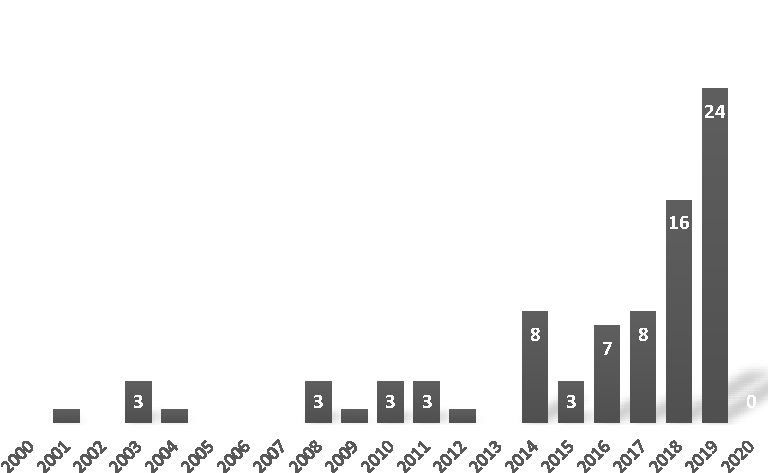
\includegraphics[width=.6\linewidth]{images/publicationyears-aiinse}
		\caption{Papers mentioning artificial intelligence in SE major venues. }
		\label{fig:publicationyears-ai}
\end{figure}

\subsubsection{Survey analysis}
We can see in \Fig{fig:publicationyears-ai} an exponential rise of the number of papers in the last years when. This contrasts with the gradual decrease of publications focused on traceability in the same period of time we have seen before (see \Fig{fig:publicationyears-tm}).

But, the key question is where these 81 papers do recognize the importance traceability or related concepts as part of their proposal. This is not the case, out of the 81 AI related papers collected in the main venues for software engineering research, only two use some kind of traceability to address functional quality of AI-enabled system. Clearly, traceability, recognized as a strong weapon for verification and accountability enhancement, has not got much attention in new AI-enabled techniques for software engineering. 
%One combines program execution and symbolic analysis to explore the execution paths of software programusing Deep Neural Networks (DNNs). In this paper, authors formalise coverage criteria for DNNs and then develop a coherent method for performing concolic testing to increase test coverage~\cite{Sun_2018-concolic-for-RNN}. In the second paper, symbolic execution is adapted into optimization problems representing the (non-)feasibility of paths. A machine learning algorithm then solves the problems. Authors show the method helps in black-box functions calls, between others, and thus is suitable for AI-enabled systems~\cite{Li_2016-symbolic-execution-feasibility}.

%\ugh{Yet AI explainability crisis would benefit from better traceability.}

%\textbf{Conclusion.} 
%AI is used for many things, including traceability. But in the software engineering realm, traceability is anything but used to aid and augment AI explainability.
%The inherent ability of artefacts to link which each others and to visualize these links explicitly is directly related to the time passed in validation and verification (inspection). We envision that explainability and accountability would gain at putting traceability as a core quality - of software development in general, and AI-enabled software in particular, and we call for more work in this area.


\subsection{Conclusion}\label{sec:conclusion}

Our survey reveals the continuous interest in traceability even if, often, is considered as a second class citizen. Our analysis also highlights several aspects of current traceability methods that should be further developed, especially if we want to use traceability techniques to improve ongoing AI explainability initiatives. 

To reach these conclusions we have conducted two surveys. The first one focused on all the works devoted to traceability methods and techniques while the second one looked at the increasing number of papers proposing AI techniques to solve software engineering problems to see if those works were integrating (or not) explainability concerns. They do not\footnote{We see the application of AI to automatically identify new traces, e.g.~\cite{clelandhuang2014-traceability-trends-and-futurte-direction} but not the opposite, i.e. the use of traceability to help explain AI components}, which makes this traceability survey even more relevant. 

Moreover, we argue that our feature model helps map the research area and will help understand and standardize traceability approaches and theories. This should help understand, compare and evaluate new traceability proposals. Indeed, there is a prominent call for generalization and standardization~\cite{wohlrab2020-traceability-organization-process-culture} in this field. Gaps between traceability-related research subfields could be better filled in with a common language bringing better communication.

We put a peculiar focus on the distinction between the modeling of traceability and the use of trace links and support our claims with two surveys. The first shows actual trends in traceability literature figuring a prominent call for generalization and standardization~\cite{wohlrab2020-traceability-organization-process-culture}. Current limitations are bond by technical, conceptual, and cultural gaps between research fields that could be fill in with a common language for a better communication. We argue that our feature model helps map the research area and will help understand and standardize traceability approaches and theories. The second survey shows that traceability, recognized as a strong weapon for verification and accountability enhancement, has not got much attention in AI-enabled software engineering. Instead, most work aiming to augment the automation level of traceability offer technical improvement in the automated derivation of links between artefacts of heterogeneous nature - and more specifically text artefacts~\cite{clelandhuang2014-traceability-trends-and-futurte-direction}.
We see this as a urgent call for more work on traceability for the explainability of AI.




%

\subsection{Qualities of research proposals}
\begin{figure*}[h]
	\centering
	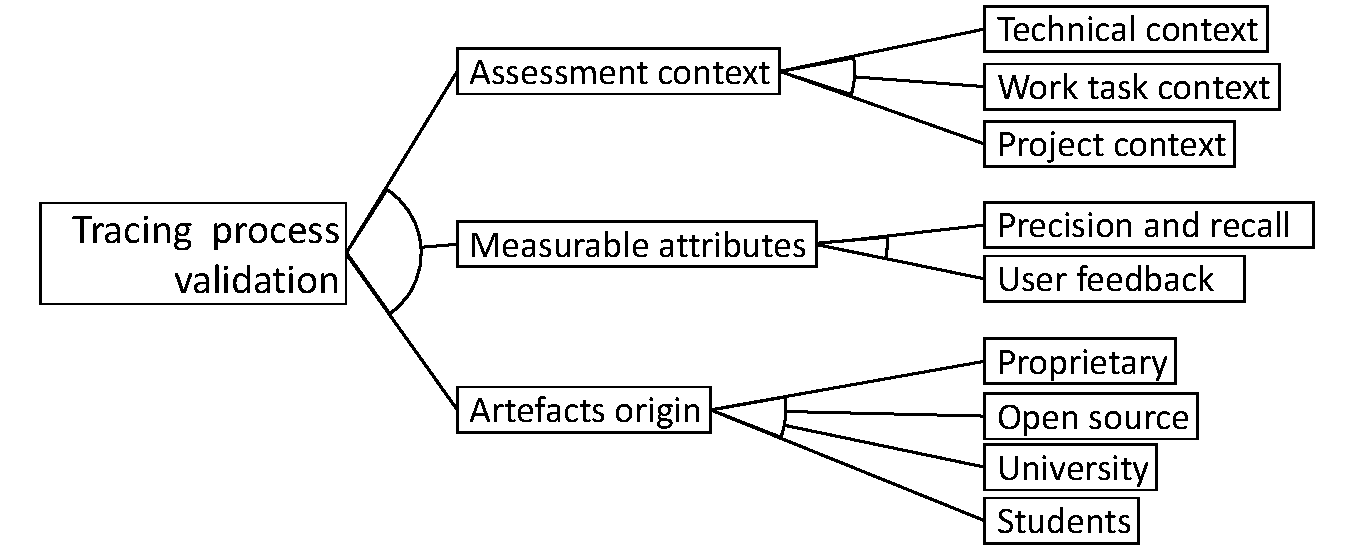
\includegraphics[width=.65\linewidth]{images/fm-quality}
	\caption{Quality measurement of traceability, research work, processes and products.}
	\label{fig:fm:quality}
\end{figure*}
\eb{I don't know where to put this.}


\subsection{Artefacts origin}
Mainly onpen source and/or academic projects.
Famous industry case: Nejati, on design slicing for SysML requirement tracing. \ugh{Unfortunately, technical assessment (to be verified)}.


\subsection{Measurable attributes} 
Regarding the performance of retrieval systems, an hegemonic predilection remains toward Recall (completeness of retrieval) and Precision (purity of retrieval) measurement alone. P\&R (and derivates) is a direct quantification allowing the comparison with closely related technical contributions, but fails to consider the overall evaluation of traceability mean and usefulness in a broader picture \ugh{(the breadth of pictures is depicted in "Evaluation context")}.

\subsection{Evaluation context} \textbf{Technical context:} Optimisation against Precision\&Recall (only). Comparison with SoA (technical as well).
\textbf{Work task context:} Trace accuracy, relevancy. By means of vetting, dashboards. Asking for a human feedback (Survey, interview, Likert scale).
\textbf{Project context:} Evaluation of traceability impact on a broader quality evaluation. Traceability process maturity correlated to liability of other quality evidences. Comparison against multifactorial experiment configurations.





%\bibliographystyle{spbasic}      % basic style, author-year citations
%\bibliographystyle{spmpsci}      % mathematics and physical sciences
%\bibliographystyle{spphys}       % APS-like style for physics
\bibliographystyle{utils/plainnatnourl}
%\setcitestyle{numbers}
\bibliography{bib/strings-abbr,bib/trace-and-models,bib/uoc2020_tracea,bib/list-aise}

%\renewcommand{\refname}{Survey selection}  % for documentclass article
%\renewcommand{\bibname}{Selected reading} % for documentclass book or report

% _appendix.bbl is generated by running latex and bibtex on _appendix.tex
%\documentclass{article}


\begin{document}

\bibliographystyle{plain}
\bibliographystyle{../utils/spbasic}


\cite{lohar2013,hayes2006,Gotel2012,li2013ontologybasedTraceRetrieval,guo2013expertSystemInTraceabilityDSL,tekinerdogan2007-metamodel-for-tracing-concers-accross-life-cycle,poshyvanyk2007,keenan2012-workbench-for-traceability,florez2019-finegrained-req2code,rempl2014-conformance-of-traceability-to-guidelines,rath2018-guo-augmenting-incomplete-traces,bonde2006-different-levels-of-abstraction,tinnes2019-improving-art-reuse-with-traceability,seiler2019-comparing-trac-through-IR-Commits-Logs,farrar2019-comparing-stemming-technics,ghaisas2019-traceability-for-a-knowledge-driven-SW,rahimi2019-Evolving-trace-req2source,lian2019-Traceability-reveals-quality-in-source,shin2015-guidelines-benchmark-auto-traceability,li2013-trace-matrix-analyzer,nejat2012-traceability-sysml-safety-certification,gannous2019-Certification-into-Model-based-Testing-for-Safety-Critical-Systems,azevedo2019-traceability-metamodel-and-reference-model,tran2011-vbTrace-view-based-MDD-processdriven-SOAs-traceability,goknil2014-change-impact-analysis-for-requirement-metamodel,fittkau2013-explorviz-Trace-Visualization,borg2014-SmS-IR-for-traceability,post2009-link-functional-req-to-verification,guo2017-semantically-enhanced-tracebility-deep-learning,rutle2018-MT-coevolution-with-traceability-and-graph-transfo,amar2013-model-coevolution-uding-traceability,wenzel2007-Tracing-model-elements,santiago2013traceability-in-MDE,aranega2011-trace-for-mutation-analysis-in-model-transformation,seibel2010-dynamic-hierarchical-models-comprehensive-traceability,schwarz2010-graph-based-traceability,paige2010-MDE-Traceability-classifications,helming2009-traceability-change-awareness,grammel2010-facet-based-traceability-data-extraction-in-MDE,vara2014-traceability-in-MDD-MTransfo,marcen2020-req2model-with-EA-ranking-train-system,ruiz18-traceME-conceptual-model-evolution,aboussoror2012-Seeing-errors-trace-visualisation,grammel2012-model-matching-for-traceability-in-MDE,mader2010-visual-tracability-modeling-language,ziegenhagen2020-tracing-life-cycles,heisig2019-generic-traceability-metamodel-end-to-end-capra,mader2008-rule-based-maintenance-post-requirements-traceability,borillo1992-linguistic-engineering-to-spacial-SE,antoniol2002-tracing-code-documentation-links,marcus2003-latent-semantic-indexing-for-traceability-LSI,mcmillan2009-combining-text-and-structural-analysis-for-traceability,badreddin2014-req-traceability-model-based-approach,panichella2013-using-structural-information-to-improve-IR-traceability,laghouaouta2017-model-composition-tracaebility,dosimont2014-eficient-analysis-methodology-for-huge-application-traces,anquetil2010-model-driven-tracea-for-SPL,diaz2015-tracing-variability-from-features-to-product-line-SPL,paige2011-traces-in-moel-driven-engineering,drivalos2009-engineering-DSL-for-traceability,gallina2014-model-driven-certification-method-for-process-compliance,asuncion2010-software-traceability-with-topic-modeling,bouillon2013-survey-on-usage-scenario-requirements-traceability-in-practice,clelandHuang2012-trace-queries-safety-requirements-assurance,dietrich2013-learning-efective-query-transformation-for-enhanced-req-trace-retrieval,li2012-which-visualization-in-this-context,mader2012-visual-language-for-traceability-queries,mader2009-motivation-matters-in-traceability-practitioner-survey,mader2013-strategic-traceability-for-safety-critical-projects,panis2010-req-traceability-deployment-in-commercial-engineering-organisation,spanoudakis2004-rule-based-generation-of-req-traceability-relations,vonknethen2002-change-oriented-req-traceability-evolution-of-embedded-systems,kuang2012-do-data-dependencies-complement-call-dependencies,yu2012-maintainging-invariant-traceability,naslavsky2007-traceability-of-MB-Testing-MT,arunthavanathan2016-traceability-with-NLP,drivalos2010-state-based-traceability,seibel2012-efficient-traceability-for-MDE,gotel1994,wohlrab2020-traceability-organization-process-culture,meinicke2017-feature-traceability,mader2007-tracing-unified-process,sotovalero2020tracebased,ziegenhagen2020-expanding-tracea-with-dynamic-tracing-data,ziegenhagen2019-developer-tool-interaction,ko2008-whyline-debugging,Bouzidi_2020,Wang_2020,Gonzalez_2019,Arcelli_2019,Markovic_2019,Guana_2017,Haidrar_2018,Diskin_2017,Filax_2017,Bunder_2017_query-for-quality,Buchmann_2015,la_Fosse_2018,Kr_mer_2016,Haidrar_2016,Cazzola_2016,Faddegon_2016,Mani_2016,Lee_2016,Di_Francescomarino_2015,Pape_2015,Ogunyomi_2015,Bauman_2015,Pace_2014,Mat__2014,Pfeiffer_2014,Inostroza_2014,Boulanger_2014,Laghouaouta_2014,Saada_2013,Szabo_2013,Santiago_2013,Rosenkranz_2013,Alhaj_2013,George_2012,van_Amstel_2012,Jim_nez_2013,2012,Sannier_2012,Graf_2012,Garces_2011,Sanchez_2011,Grosch_2011,Ono_2010,Yrj_nen_2010,Levendovszky_2010,Pfeiffer_2010,bin_Abid_2010,Goknil_2010,Dubois_2010,Naslavsky_2010,Her_2010,Morgan_2010,Grave_2010,Hegedus_2010,Dickerson_2010,Maoz_2009,Clauzel_2009,Valderas_2009,Kerstan_2008,Boskovic_2007,Olsen,Almeida_2007,Triebsees_2007,Almeida_2006,Brassel_2006,Peischl_2005,Belkadi_2006,Mason,Nilsson_1999,Corbett_1995,Borstler_1992,paige2017-changing-mde}


\bibliography{../bib/trace-and-models}

\end{document}


\end{document}
